\documentclass[12pt]{article}

% ============================ PREAMBLE ============================
\usepackage[margin=1in]{geometry}
\usepackage{setspace}
\usepackage[T1]{fontenc}
\usepackage[utf8]{inputenc}
\usepackage{csquotes}
\usepackage{graphicx}
% Add a thin border around every \includegraphics automatically
\setlength{\fboxsep}{0pt} 
\setlength{\fboxrule}{0.4pt} % border thickness
\let\oldincludegraphics\includegraphics
\renewcommand{\includegraphics}[2][]{%
  \fbox{\oldincludegraphics[#1]{#2}}%
}

\usepackage{booktabs}
\usepackage{array}
\usepackage{longtable}
\usepackage{multirow}
\usepackage{caption}
\captionsetup[longtable]{
  justification=raggedright,
  singlelinecheck=false
}
\setlength{\LTleft}{0pt}
\setlength{\LTright}{0pt}
\setlength{\LTcapwidth}{\textwidth}
\usepackage{float}
\usepackage{amsmath,amssymb}
\usepackage{xcolor}
\usepackage{hyperref}
\graphicspath{{Graph_output_results/}{Study_exhibits/}}
\usepackage{grffile}
\usepackage{xltabular}
\usepackage{parskip}
\hypersetup{
    colorlinks=true,
    linkcolor=black,
    citecolor=blue,
    urlcolor=blue
}

% ---- Bibliography (Harvard / author-year via biblatex + biber) ----

\usepackage[
    backend=biber,
    style=authoryear,
    maxcitenames=2,
    maxbibnames=99,
    uniquename=false,
    uniquelist=false,
    natbib=true
]{biblatex}
\addbibresource{Community Moderation Experiment.bib}   % <-- bixtext file name

% Nicer caption formatting
\captionsetup{font=small,labelfont=bf,labelsep=period,justification=raggedright,singlelinecheck=false}


\title{%
\begin{minipage}{0.88\textwidth}
\centering
\Large
Motivated Moderation: Political Content and Partisan Opposition Result in Stricter Civility Enforcement in Community Moderation Settings
\end{minipage}
}

\author{Rehan A. Mirza\thanks{Annenberg School for Communication, University of Pennsylvania.}}
\date{}

\begin{document}

\maketitle
% ============================ ABSTRACT ============================
\begin{abstract}

\noindent Content moderation requires moderators to balance harm prevention with free expression, a tension that is especially acute for political incivility, where norm violations must be weighed against salient political speech. Prior work suggests that moderation decisions may be distorted by motivated partisan reasoning, yet evidence from community-driven settings, where users create and enforce rules, remains limited. This study examines whether partisan alignment biases moderation judgments in community settings.

\vspace{0.75em}


\noindent Using a $3\times2$ within-subjects survey experiment simulating a moderator queue, U.S.-based participants evaluated social media memes varying in partisan alignment (aligned vs.\ opposed) and civility (uncivil, borderline uncivil, civil), applying explicit community rules to select enforcement actions with specified consequences. Outcomes were measured across two dimensions: violation recognition (whether content should be censored) and enforcement severity (the level of action taken). By focusing on civility rather than fact-based violations, the study tests mechanisms of motivated reasoning---specifically \enquote{party promotion} and \enquote{preference gaps}---in rule-based rather than accuracy-based moderation judgments.

\vspace{0.75em}


\noindent Three findings emerge. Firstly, political content is judged more stringently than matched non-political content at civil and borderline levels, suggesting political material may arouse heightened perceptions of norm violation independent of civility. Secondly, partisan opposition significantly increases both violation recognition and enforcement severity: opposed content is more likely to be flagged as rule-violating and receives more severe enforcement than aligned content. Thirdly, this alignment effect does not vary across civility levels, indicating it operates across the full range of civil, borderline, and uncivil content, rather than only where rules are ambiguous. These findings extend research on politically motivated moderation to rule-based community settings, with implications for platform governance as major platforms increasingly delegate moderation to volunteer communities.

\end{abstract}

\vspace{1em}
\doublespacing 

% ============================ INTRODUCTION ============================
\section{Introduction}

Content moderation shapes the information we see online and facilitates civil conversations, making it an important component of governance for healthy online environments \parencite{myerswestCensoredSuspendedShadowbanned2018,matiasCivicLaborVolunteer2019}. Moderators make innumerable decisions about what content users see, and what is removed, including content that violates platform terms of service or community norms. This may include hate speech, antagonization, threatening language, harassment, or insulting language \parencite{bonottiUnderstandingCivility2021,gervaisIncivilityInvalidityEvaluating2025,leibmannRedditRulesRulers2025}. Uncivil content can represent a departure from norms of politeness, mutual respect, and shared commitments in political discourse \parencite{bonottiUnderstandingCivility2021}. Although conflict is an important component of democratic deliberation, Americans often respond unfavorably to uncivil political conflict, which can produce negative affect, distrust, polarization, and exaggerated perceptions of extremity amongst political opponents \parencite{mutzInYourFacePoliticsConsequences2015}. Judgments on whether this content is harmful, whether it breaches platform rules, and what actions to take in response are inherently subjective \parencite{diakopoulosQualityDiscourseOnline2011,kozyrevaResolvingContentModeration2023}. This represents a central governance challenge: though such content can undermine the norms communities rely on to sustain constructive participation, removing the content too aggressively can restrict legitimate free expression \parencite{kozyrevaResolvingContentModeration2023}. This challenge is particularly acute in political contexts where incivility is pervasive \parencite{mutzInYourFacePoliticsConsequences2015}.

Previous studies suggest that moderation decisions may be influenced by political partisanship \parencite{lindnerAlienableSpeechIdeological2009,appelPartisanConflictContent2023a,kozyrevaResolvingContentModeration2023,solomonIllusoryInterpartyDisagreement2024}. \textcite{appelPartisanConflictContent2023a} identify three mechanisms for partisan influence on moderator judgments: a) the \enquote{fact gap}, that partisanship hinders the ability for individuals to detect misinformation when it is aligned with their political views; b) \enquote{party promotion}, a desire to leave misinformation online when it benefits one's own party or denigrates another party, and to remove misinformation with the opposite effect; and c) a \enquote{preference gap}, where partisans disagree about whether content should be removed due to internalized preferences, such as identity, core values, or internalization of elite cues. They find strong partisan differences in stated preferences of U.S.\ citizens around platform moderation of political headlines, driven by motivated reasoning that extends beyond perceptions of fact. Related work finds partisans agree on what hate speech to censor but differ on how much, driven by free speech values rather than disagreements about which groups warrant protection \parencite{solomonIllusoryInterpartyDisagreement2024}.

With platforms accused of bias in moderation \parencite{moslehDifferencesMisinformationSharing2024}, bottom-up, community-led moderation---where users create and enforce rules \parencite{leibmannRedditRulesRulers2025}---has been proposed as an alternative. Proponents argue decentralized moderators, \enquote{intimately aware} of community norms, are less likely to inappropriately restrict content \parencite{marrazzoFederalistsInternetWhat2023}. This view is rooted in the principle of \enquote{network communitarianism}; that online communities function as key stakeholders whose norms should guide moderation approaches \parencite{kozyrevaResolvingContentModeration2023}. While platform-level moderation has been studied considerably \parencite{chenNeutralBotsProbe2021,moslehDifferencesMisinformationSharing2024,hallinanblakeAspirationalPlatformGovernance2025}, partisan decision-making in community moderation remains relatively unexplored.

This study tests whether partisan alignment influences moderator judgments when evaluating the civility of memes in a community forum. In contrast to prior work focused on news headlines, misinformation or hate speech \parencite{appelPartisanConflictContent2023a,kozyrevaResolvingContentModeration2023,solomonIllusoryInterpartyDisagreement2024}, this study examines rule-based judgments about civility in a lower-stakes meme context. Participants evaluated political posts that varied in alignment with their stated party preference and in civility, then selected whether and how to enforce the provided community rules. They also evaluated non-political posts that varied in civility as a baseline. This design examined whether political opposition and civility independently shaped moderation judgments, and whether the effect of alignment varies across civility levels. The approach aims to capture moderation behaviors, asking participants to select enforcement actions with specified consequences, rather than stated preferences about content appropriateness.

Moderator perceptions were measured across two dimensions: \enquote{violation recognition}, whether content was judged to break the rules, and \enquote{enforcement severity}, the degree of action to take in response, building on prior approaches \parencite{kozyrevaResolvingContentModeration2023,solomonIllusoryInterpartyDisagreement2024}. I test whether increased incivility and partisan opposition shape both outcomes, and whether the alignment effect varies across civility levels. I also compare political posts with non-political posts at matched civility levels to explore whether political content itself is associated with more stringent moderation.

This study makes three contributions. Firstly, it shows that political content is moderated more harshly than non-political baseline content, even when posts are civil or only borderline uncivil. Secondly, it shows that politically opposed content receives harsher moderation judgments (than aligned content) across both violation recognition and enforcement severity. Thirdly, it finds that this alignment effect does not vary significantly across civility levels. This suggests that alignment effects may reflect more general differences in how participants respond to politically aligned versus opposed content, rather than effects that only emerge when rule boundaries are ambiguous.

The rest of this paper is organized as follows: I outline the theoretical foundations and hypotheses, followed by methodology and presentation of results. I conclude with a discussion of the findings, including implications for policy, limitations, and directions for further research.

% ============================ THEORY ============================
\section{Theoretical foundations}

This study examines how partisan alignment influences content moderation in a $3\times2$ within-subjects survey experiment simulating a community forum. Participants moderate six social media posts that vary in partisan alignment with the respondent (aligned vs.\ opposed) and civility (uncivil, borderline uncivil, and civil). They are asked to decide whether the content they see violates these rules, and what enforcement action to take.

Past research suggests that clearly articulated community norms help guide user behavior and reduce unruly conduct \parencite{matiasCivicLaborVolunteer2019,leibmannRedditRulesRulers2025}. If these norms are made explicit, they can provide a shared reference point for moderators to assess when content crosses civility boundaries, even when applying those rules remains subjective. Therefore, the baseline expectation is that incivility itself drives violation recognition and enforcement severity:

\begin{quote}
\textbf{H1a:} More uncivil content is more likely to be judged as a violation of community rules.

\textbf{H1b:} More uncivil content receives more severe enforcement actions.
\end{quote}

The expected direction of the civility effect is anticipated to hold regardless of alignment; whether the magnitude varies across alignment conditions is tested under H3.

Past research, however, also emphasizes the effects of partisan alignment in content moderation decisions \parencite{lindnerAlienableSpeechIdeological2009,appelPartisanConflictContent2023a,kozyrevaResolvingContentModeration2023,solomonIllusoryInterpartyDisagreement2024}. Mechanisms such as \enquote{party promotion} (the strategic preservation of aligned content) and \enquote{preference gaps} (differing internalized preferences) can lead individuals to apply more lenient standards to aligned content and stricter standards to opposed content \parencite{appelPartisanConflictContent2023a}. These mechanisms may differentially influence moderation decisions depending on the judgment made. I theorize that violation recognition is primarily a values-driven judgment shaped by preference gaps, where internalized differences for what constitutes acceptable discourse lead partisans to perceive violations differently based on alignment. Correspondingly, enforcement severity can also carry stronger strategic implications tied to party promotion, because actions taken influence the extent to which political opponents face meaningful consequences for violative content.

Consequently, partisan alignment is expected to exert independent influence on both outcomes:

\begin{quote}
\textbf{H2a:} Aligned content is less likely to be judged as a violation of community rules.

\textbf{H2b:} Aligned content receives less severe enforcement actions.
\end{quote}

Civility levels may condition the size of the alignment effect. In this study, \enquote{borderline uncivil content} is used to represent greater interpretive ambiguity: relative to \enquote{uncivil} and \enquote{civil} content, which may be cleanly interpreted as \enquote{unacceptable incivility} or \enquote{legitimate partisan criticism} respectively, it sits closer to the boundary between these interpretations. This boundary is itself a subjective judgment. \textcite{solomonIllusoryInterpartyDisagreement2024} show that even when partisans broadly agree on which content warrants censorship, they may differ in how much enforcement is appropriate, reflecting differences in underlying free-speech values. This suggests that alignment effects may vary across civility levels if ambiguity provides participants more room to apply different standards to aligned and opposed content. However, alignment may also operate more uniformly if participants bring stable preferences to political content regardless of civility level. I therefore test whether the effect of partisan alignment varies across civility levels.

\begin{quote}
\textbf{H3a:} The effect of partisan alignment on violation recognition varies across civility levels.

\textbf{H3b:} The effect of partisan alignment on enforcement severity varies across civility levels.
\end{quote}

% ============================ METHODS ============================
\section{Methods}

\subsection{Participants}

Participants were recruited from Forthright's online survey panel and pre-screened to obtain a balanced sample of self-identified Democrats and Republicans ($N = 254$ total participants; 139 Democrats; 115 Republicans). Independents were excluded to ensure a clear operationalization of partisan alignment. One duplicate respondent entry was excluded. Respondents also provided demographic information which is summarized in the \hyperref[sec:descriptive]{Appendix} to describe the sample.

\subsection{Study design}

The study employed a $3\times2$ within-subjects design, manipulating:

\begin{itemize}
    \item \textbf{Partisan alignment:} Aligned vs.\ opposed to a participant's stated political party preference.
    \item \textbf{Civility:} Civil vs.\ borderline uncivil vs.\ uncivil.
\end{itemize}

Alignment was manipulated by presenting memes with \enquote{left-leaning} (\enquote{aligned} for Democrats, \enquote{opposed} for Republicans) and \enquote{right-leaning} content (\enquote{aligned} for Republicans, \enquote{opposed} for Democrats). \enquote{Right-leaning} content included criticism of Democrats, Democrat-aligned figures such as Zohran Mamdani and Joe Biden, and Democrat associated controversies and policies. \enquote{Left-leaning} wording included criticism of Republicans, Donald Trump, and Republican associated controversies and policies.

\begin{figure}[H]
    \centering
    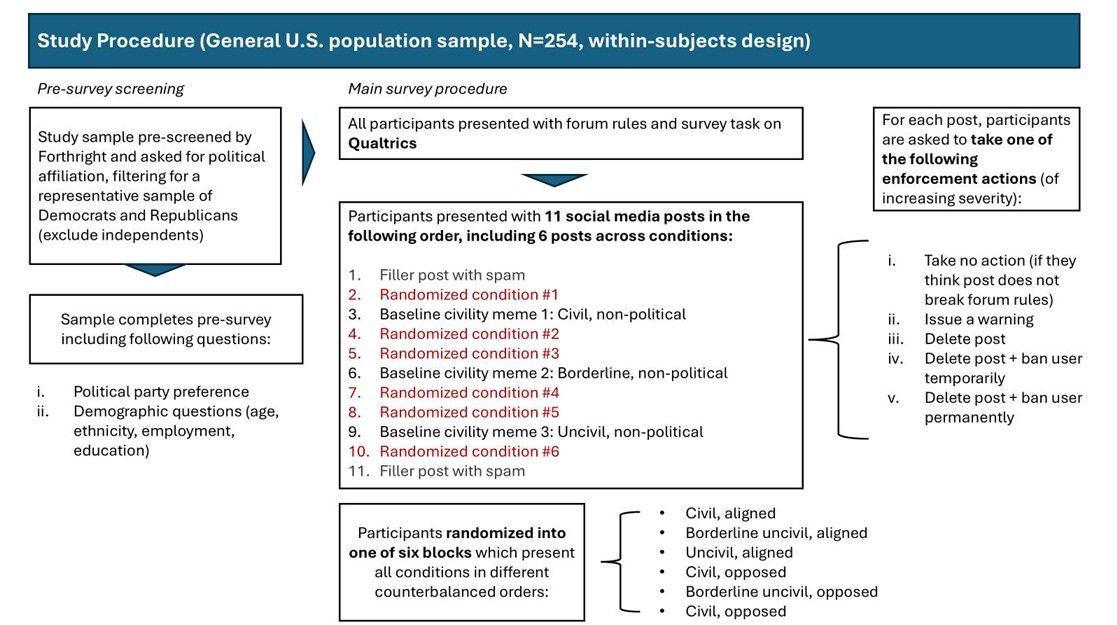
\includegraphics[width=\linewidth]{Study_Exhibits/Fig_1_Study_Procedure.jpg}
    \caption{Study procedure.}
    \label{fig:study_procedure}
\end{figure}

Civility manipulations followed the scale employed by \textcite{solomonIllusoryInterpartyDisagreement2024}: civil discourse as \enquote{criticism of the opposition}, borderline uncivil as insulting language (e.g., \enquote{illiterate}, \enquote{idiots}, \enquote{just plain stupid}) and uncivil as \enquote{dehumanization and incitement} (e.g., comparisons to animals, violence against political opponents).

After pre-screening for participant information by the survey provider and an introductory screen presenting the task, participants were shown the community rules and moderator instructions, presented in Figure~\ref{fig:comm_rules} in the Appendix. The rules included requirements that \enquote{posts must be memes}, to \enquote{remain civil and respectful}, and that posts should \enquote{not contain spam or advertisements}. Each participant reviewed 11 posts: six experimental conditions (all combinations of 3 civility $\times$ 2 alignment levels), three non-political posts with varying civility levels, and two spam fillers. Figure~\ref{fig:ordermix} in the Appendix provides a visual example of the set of items viewed in Order~1, and Table~\ref{tab:memes} provides a full list of memes, topics and content by condition for each order block.

Following the logic of a prior approach \parencite{mutzEffectsInYourFaceTelevision2007}, respondents were randomly assigned to one of six counterbalancing blocks that rotated the six conditions across presentation positions and meme topics. The content and positions of the filler and non-political posts were constant across blocks. This ordering approach, presented in Table~\ref{tab:counterbalance}, ensured that each condition appeared in each sequence position across the full sample, while avoiding the increase to 36 orderings that a full Latin-square design would require for $3\times2$ factors. However, condition-order pairings were not fully balanced, and the design therefore cannot rule out all order or topic effects. I address this limitation through an order-block robustness analysis reported below. As a final note on design, the study was not preregistered, the implications of which are discussed in study limitations.

\vspace{0.75em}


% -------- TABLE 1: Counterbalancing (transposed to fit page width) --------
% Positions are rows; each order block has a Topic column and a Condition column.
\begin{table}[H]
    \centering
    \caption{Counterbalancing of political conditions across the six randomized block orders. Each cell pairs the meme \emph{topic} (T1--T6) with the experimental \emph{condition} (civility $\times$ alignment) shown at that position.}
    \label{tab:counterbalance}
    \footnotesize
    \setlength{\tabcolsep}{4pt}
    \renewcommand{\arraystretch}{1.2}
    \begin{tabular}{@{}l l l l l l l@{}}
        \toprule
        \textbf{Position} & \textbf{Order 1} & \textbf{Order 2} & \textbf{Order 3} & \textbf{Order 4} & \textbf{Order 5} & \textbf{Order 6} \\
        \midrule
        Position 1 & T1: Civil-L     & T3: Civil-R      & T5: Bord.-L      & T1: Bord.-R      & T3: Uncivil-L    & T5: Uncivil-R \\
        Position 2 & T2: Civil-R     & T4: Bord.-L      & T6: Bord.-R      & T2: Uncivil-L    & T4: Uncivil-R    & T6: Civil-L \\
        Position 3 & T3: Bord.-L     & T5: Bord.-R      & T1: Uncivil-L    & T3: Uncivil-R    & T5: Civil-L      & T1: Civil-R \\
        Position 4 & T4: Bord.-R     & T6: Uncivil-L    & T2: Uncivil-R    & T4: Civil-L      & T6: Civil-R      & T2: Bord.-L \\
        Position 5 & T5: Uncivil-L   & T1: Uncivil-R    & T3: Civil-L      & T5: Civil-R      & T1: Bord.-L      & T3: Bord.-R \\
        Position 6 & T6: Uncivil-R   & T2: Civil-L      & T4: Civil-R      & T6: Bord.-L      & T2: Bord.-R      & T4: Uncivil-L \\
        \bottomrule
    \end{tabular}

    \vspace{2pt}
    {\footnotesize\itshape L = left-leaning, R = right-leaning; Bord.\ = borderline uncivil.}
\end{table}

\subsection{Dependent variable measures}

For each post, participants selected one option from a five-point scale reflecting increasing severity, based on approaches in prior studies \parencite{kozyrevaResolvingContentModeration2023,solomonIllusoryInterpartyDisagreement2024}:

\begin{enumerate}
    \item Take no action
    \item Issue a warning
    \item Delete the post
    \item Delete the post and temporarily ban the user
    \item Delete the post and permanently ban the user
\end{enumerate}

Selecting \enquote{take no action} indicated that the participant did not perceive the post as violating community rules; all other responses indicated that the participant perceived a violation and selected an enforcement action.

The study employed two dependent variable measures derived from this response scale. Firstly, \enquote{violation recognition} was coded as a binary indicator of whether the participant perceived rule violation: $0 =$ \enquote{take no action} and $1 =$ any enforcement action (i.e., options 2--5). Secondly, enforcement severity retained the full ordinal scale of action intensity, coded from $0 =$ \enquote{take no action} to $4 =$ \enquote{delete the post and permanently ban the user}. Consequently, violation recognition captures whether participants judged a post to warrant moderation, whereas enforcement severity captures the overall stringency of the selected moderation response. All experimental stimuli were non-spam memes, so enforcement decisions on non-spam posts were interpreted as responses to the civility rule rather than to the meme-format or spam rules.

\subsection{Non-political conditions and filler content}

Three non-political memes varied by civility using the same levels defined by \textcite{solomonIllusoryInterpartyDisagreement2024}. These posts established a non-political behavioral baseline, allowing a comparison of how participants responded to the same civility levels in the absence of political content. Two spam posts were also included as fillers but not analyzed. Both the non-political conditions and filler items were designed to enhance ecological validity, mirroring a diversity of content in a memes forum that is not necessarily political, and reduce the risk of demand effects where participants infer the study is focused on political memes. Figure~\ref{fig:spam_nonpol} in the Appendix displays exhibits for the full set of non-political baseline and filler items viewed by all participants.

\subsection{Analysis}

Analysis was conducted in R (version 4.5.2) in three stages. Firstly, I summarized the sample and response distributions. Secondly, I constructed one-way repeated measures ANOVAs estimating the effect of civility on non-political baseline posts. Thirdly, I constructed $3\times2$ repeated-measures ANOVAs testing the effects of civility (H1a/H1b), partisan alignment (H2a/H2b), and the civility $\times$ alignment interaction (H3a/H3b).

To establish the non-political baseline effect, I analyzed three non-political posts using a one-way repeated-measures ANOVA with civility (civil vs.\ borderline uncivil vs.\ uncivil) as a within-subjects factor. This analysis estimates whether the civility manipulation produces the hypothesized graduation in violation recognition and enforcement severity in the absence of political content. The primary analysis examined the six political conditions using a $3\times2$ repeated-measures ANOVA for each dependent variable, with civility and partisan alignment as within-subjects factors. Mauchly's sphericity test was applied to all ANOVAs, with Greenhouse-Geisser corrections applied where appropriate \parencite{blancaRepeatedMeasuresANOVA2023}. Presented error bars in the results section represent 95\% between-subjects confidence intervals.

I also conducted two secondary exploratory studies. Firstly, I compared responses to political and non-political posts at matched civility levels to assess whether political content was associated with elevated violation recognition or enforcement severity, beyond differences attributed to the assigned civility level itself. As the non-political posts were included as baseline items rather than as a fully randomized factor, this comparison is interpreted descriptively and used to motivate future research, rather than to confirm an a priori hypothesis. Secondly, I estimated the political condition ANOVAs separately for Democrat and Republican respondents to explore whether alignment effects differed across partisan groups. These subgroup analyses are treated as exploratory because the study was not powered to explicitly test differences between partisan groups.

Finally, I conducted an order-block robustness analysis to assess whether the ordering approach affected the main results. This analysis estimated $3\times2$ mixed ANOVAs for each dependent variable, with civility and partisan alignment as within-subjects factors and the order block as a between-subjects factor. The purpose of this analysis was to assess whether the main alignment and civility effects were stable across the six presentation orders, not to validate randomization or test demographic balance.

% ============================ RESULTS ============================
\section{Results}

\subsection{Non-political baseline: civility shifts moderation decisions}

Figure~\ref{fig:nonpol_VR_ES} presents outcome measures for the non-political memes. Participants were by far the most likely to judge uncivil content as rule-breaking (91.7\% of cases), followed by borderline content (33.5\% of cases), and were least likely to judge civil content as rule-breaking (8.7\% of cases). Consistent with these findings, there was a large main effect of civility on violation recognition: $F(1.82, 461.14) = 452.78$, $p<0.001$ (Greenhouse-Geisser corrected). A similar pattern held for enforcement severity. Enforcement actions were most severe for uncivil posts ($M = 2.54$), followed by borderline posts ($M = 0.52$), and minimal for civil posts ($M = 0.12$). Correspondingly with these findings, there was a large main effect of civility on enforcement severity: $F(1.59, 402.16) = 612.56$, $p<0.001$ (Greenhouse-Geisser corrected). These findings support \textbf{H1a/H1b}, establishing that civility shifts both outcomes as expected, absent of political content.

\begin{figure}[H]
    \centering
    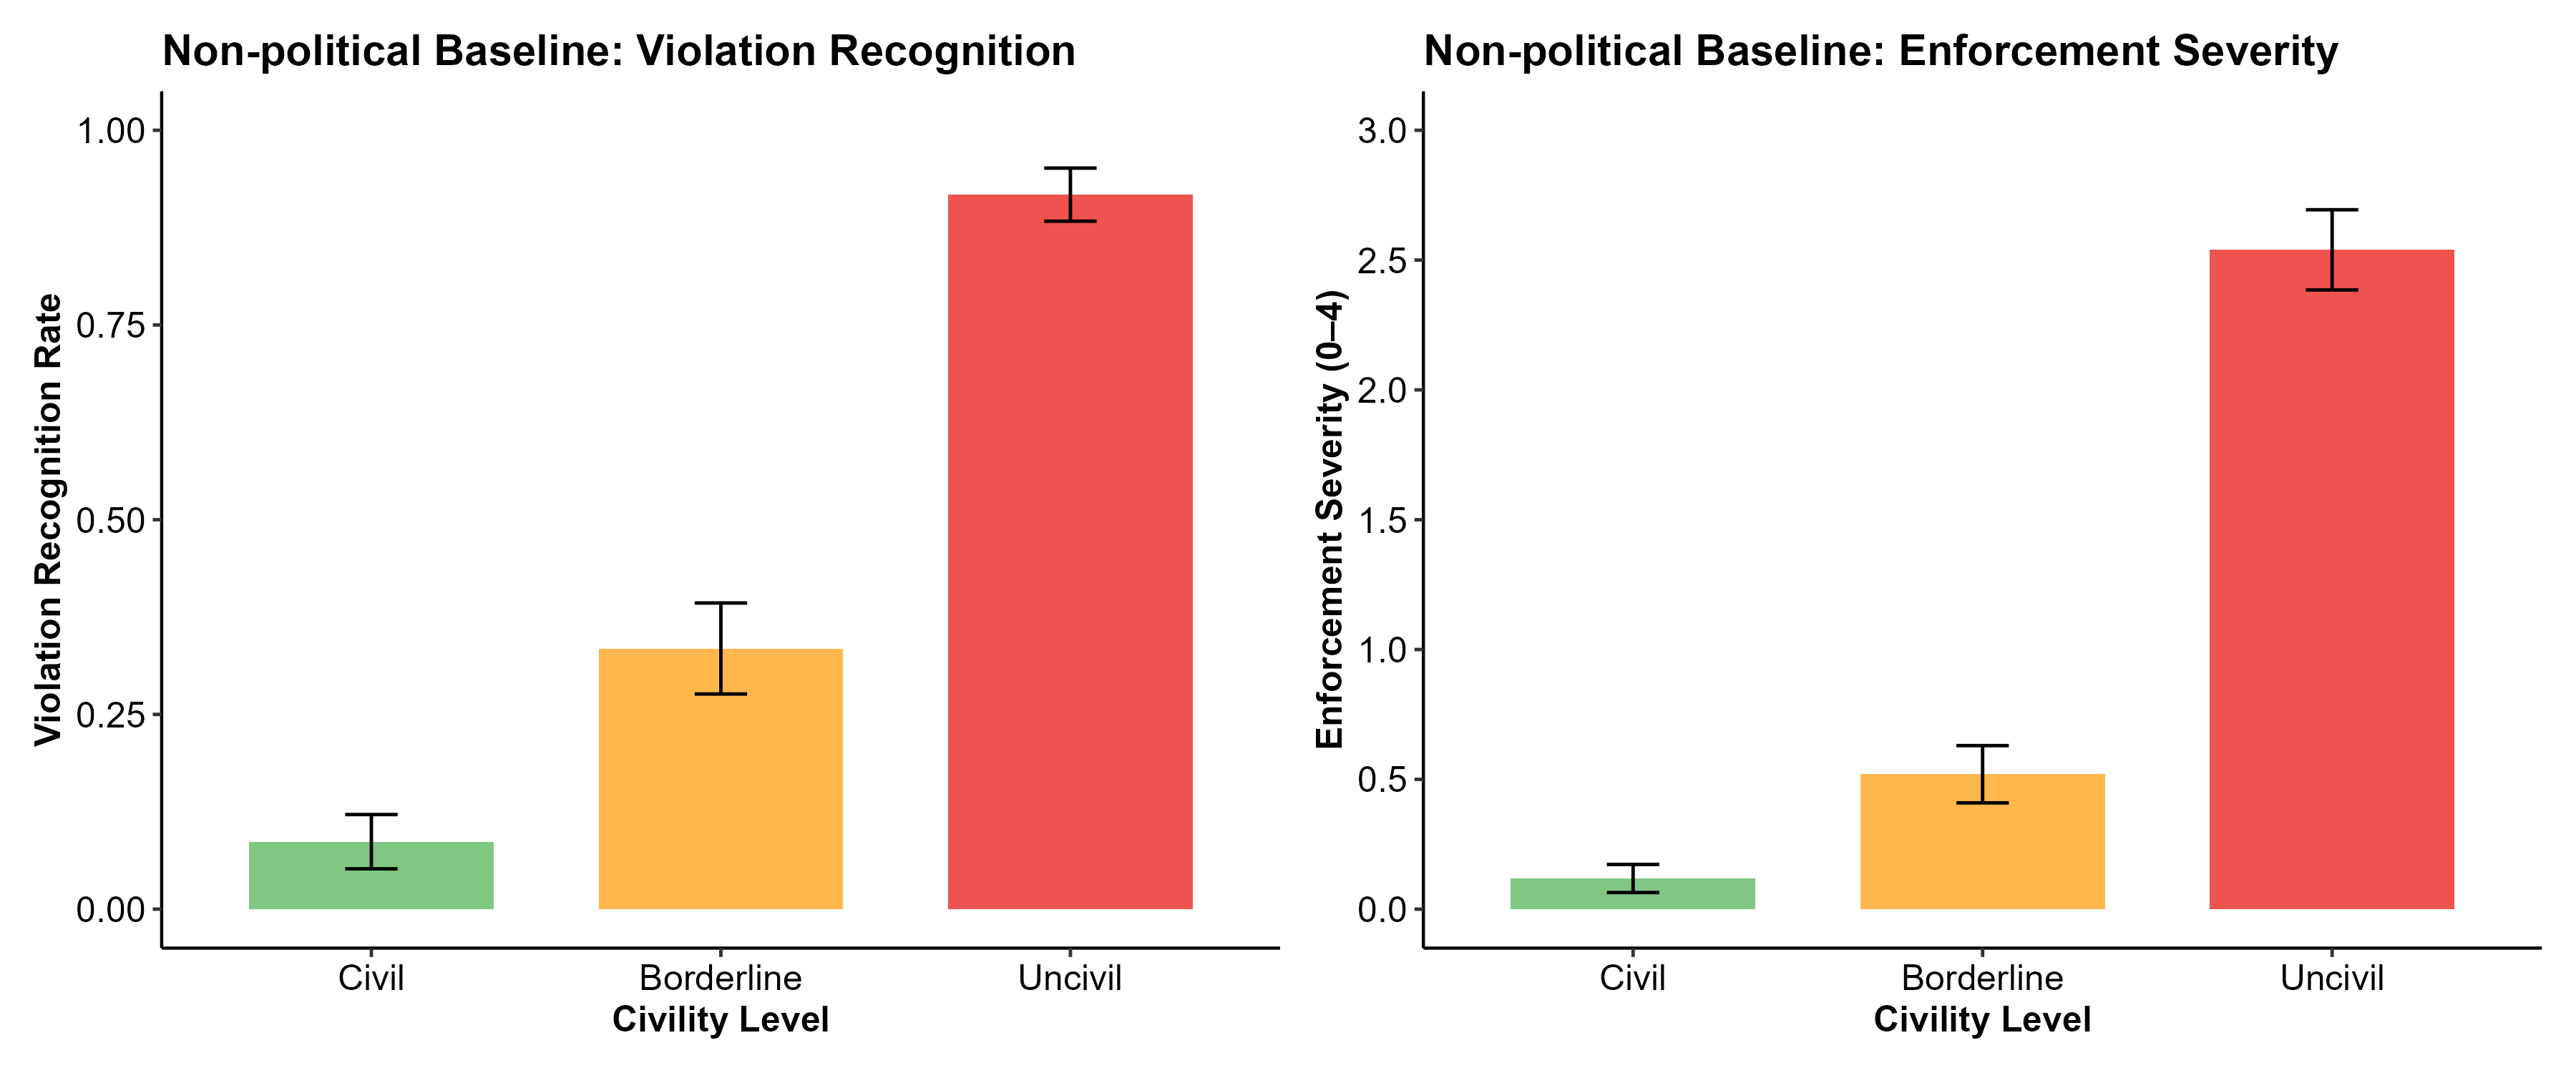
\includegraphics[width=\linewidth]{Moderation_Results_NonPolitical.png}
    \caption{Violation recognition and enforcement severity by civility conditions (non-political baseline).}
    \label{fig:nonpol_VR_ES}
\end{figure}
\subsection{Does partisan alignment influence moderation decisions?}

Figure~\ref{fig:pol_VR_ES} presents outcome measures across the six tested political conditions. A $3\times2$ repeated measures ANOVA on political content replicated the strong civility main effect for violation recognition: $F(1.98, 500.14) = 172.31$, $p<0.001$, partial $\eta^2 = .405$, Greenhouse-Geisser corrected (this main effect of civility, estimated by averaging across alignment conditions, is the test of H1; whether the effect varies by alignment is tested under H3). Participants perceived violations more frequently as civility decreased: from 47.3\% of civil cases (averaged across alignment), to 62.1\% of borderline cases, to 91.3\% of uncivil cases, \textbf{supporting H1a}. Civility also had a strong main effect for enforcement severity: $F(1.80, 455.52) = 305.12$, $p<0.001$, partial $\eta^2 = .547$, Greenhouse-Geisser corrected. Participants selected increasingly severe actions from civil ($M = 0.96$, averaged across alignment) to borderline ($M = 1.23$) to uncivil content ($M = 2.45$), \textbf{supporting H1b}.

\begin{figure}[H]
    \centering
    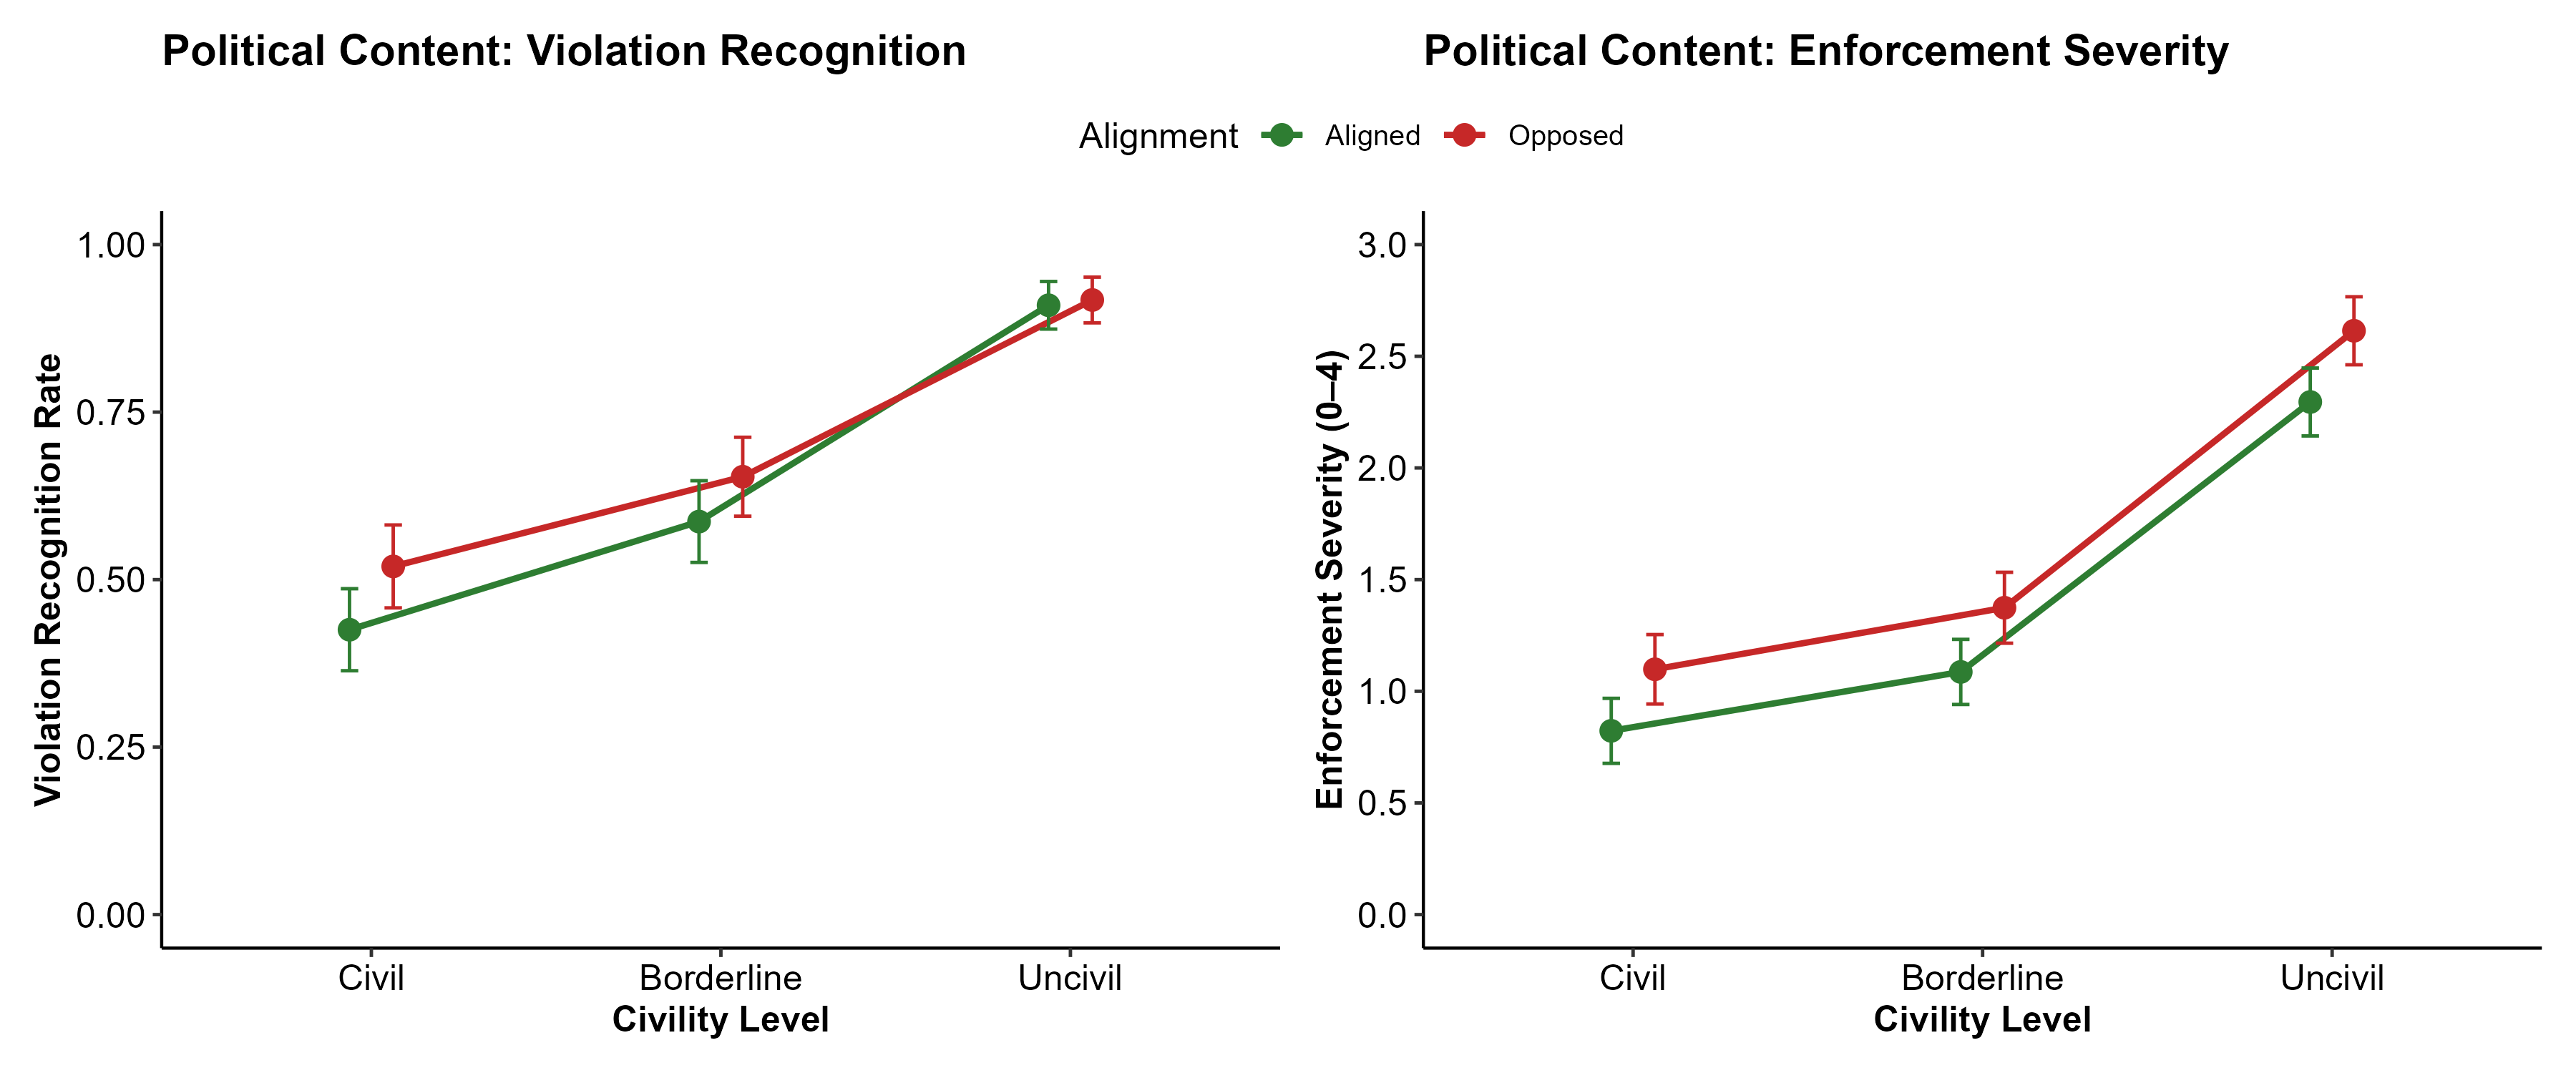
\includegraphics[width=\linewidth]{Graph_output_results/Moderation_Results_Political.png}
    \caption{Violation recognition and enforcement severity by civility and alignment for political memes.}
    \label{fig:pol_VR_ES}
\end{figure}

The ANOVA also found a significant main effect of alignment on violation recognition: $F(1, 253) = 9.81$, $p=0.002$, partial $\eta^2 = .037$. Averaged across civility levels, participants recognized violations more frequently in opposed content (69.7\% of cases) than aligned content (64.0\% of cases), \textbf{supporting H2a}. The main effect of partisan alignment was also significant for enforcement severity: $F(1, 253) = 31.99$, $p<0.001$, partial $\eta^2 = .112$. Participants also selected more severe enforcement actions for opposed content ($M = 1.69$) than aligned content ($M = 1.40$), \textbf{supporting H2b}. These findings show a consistent alignment effect in moderation judgments, with participants applying harsher judgments to politically opposed content than to aligned content.

The interaction between alignment and civility was not significant for violation recognition: $F(1.87, 472.66) = 2.31$, $p=0.104$, partial $\eta^2 = .009$, Greenhouse-Geisser corrected, nor for enforcement severity: $F(1.99, 502.32) = 0.09$, $p=0.913$, partial $\eta^2 < .001$, Greenhouse-Geisser corrected. Alignment effects on moderation decisions did not vary significantly across civility levels. Instead, the alignment effect did not vary significantly across civil, borderline uncivil, and uncivil content, providing no evidence that it was concentrated at the borderline level. Consequently, \textbf{H3a and H3b were not supported}.

\subsection{Political content was moderated more stringently than non-political content}

Figure~\ref{fig:nonpol_vs_pol} presents moderation responses to political and non-political baseline posts at matched civility levels. A repeated-measures ANOVA found a significant civility $\times$ content type interaction for violation recognition: $F(2, 506) = 78.14$, $p<0.001$, partial $\eta^2 = .236$, indicating the gap between political and non-political memes varied by civility level. Political content was substantially more likely to be judged as rule violating when posts were civil (47.3\% political vs.\ 8.7\% non-political, $+38.5$ percentage points, $p<0.001$) and borderline uncivil (62.1\% political vs.\ 33.5\% non-political, $+28.5$ percentage points, $p<0.001$). However, this gap disappeared for uncivil content, where political and non-political posts were judged as violations at similar rates (91.3\% political vs.\ 91.7\% non-political, $p=0.79$).

\begin{figure}[H]
    \centering
    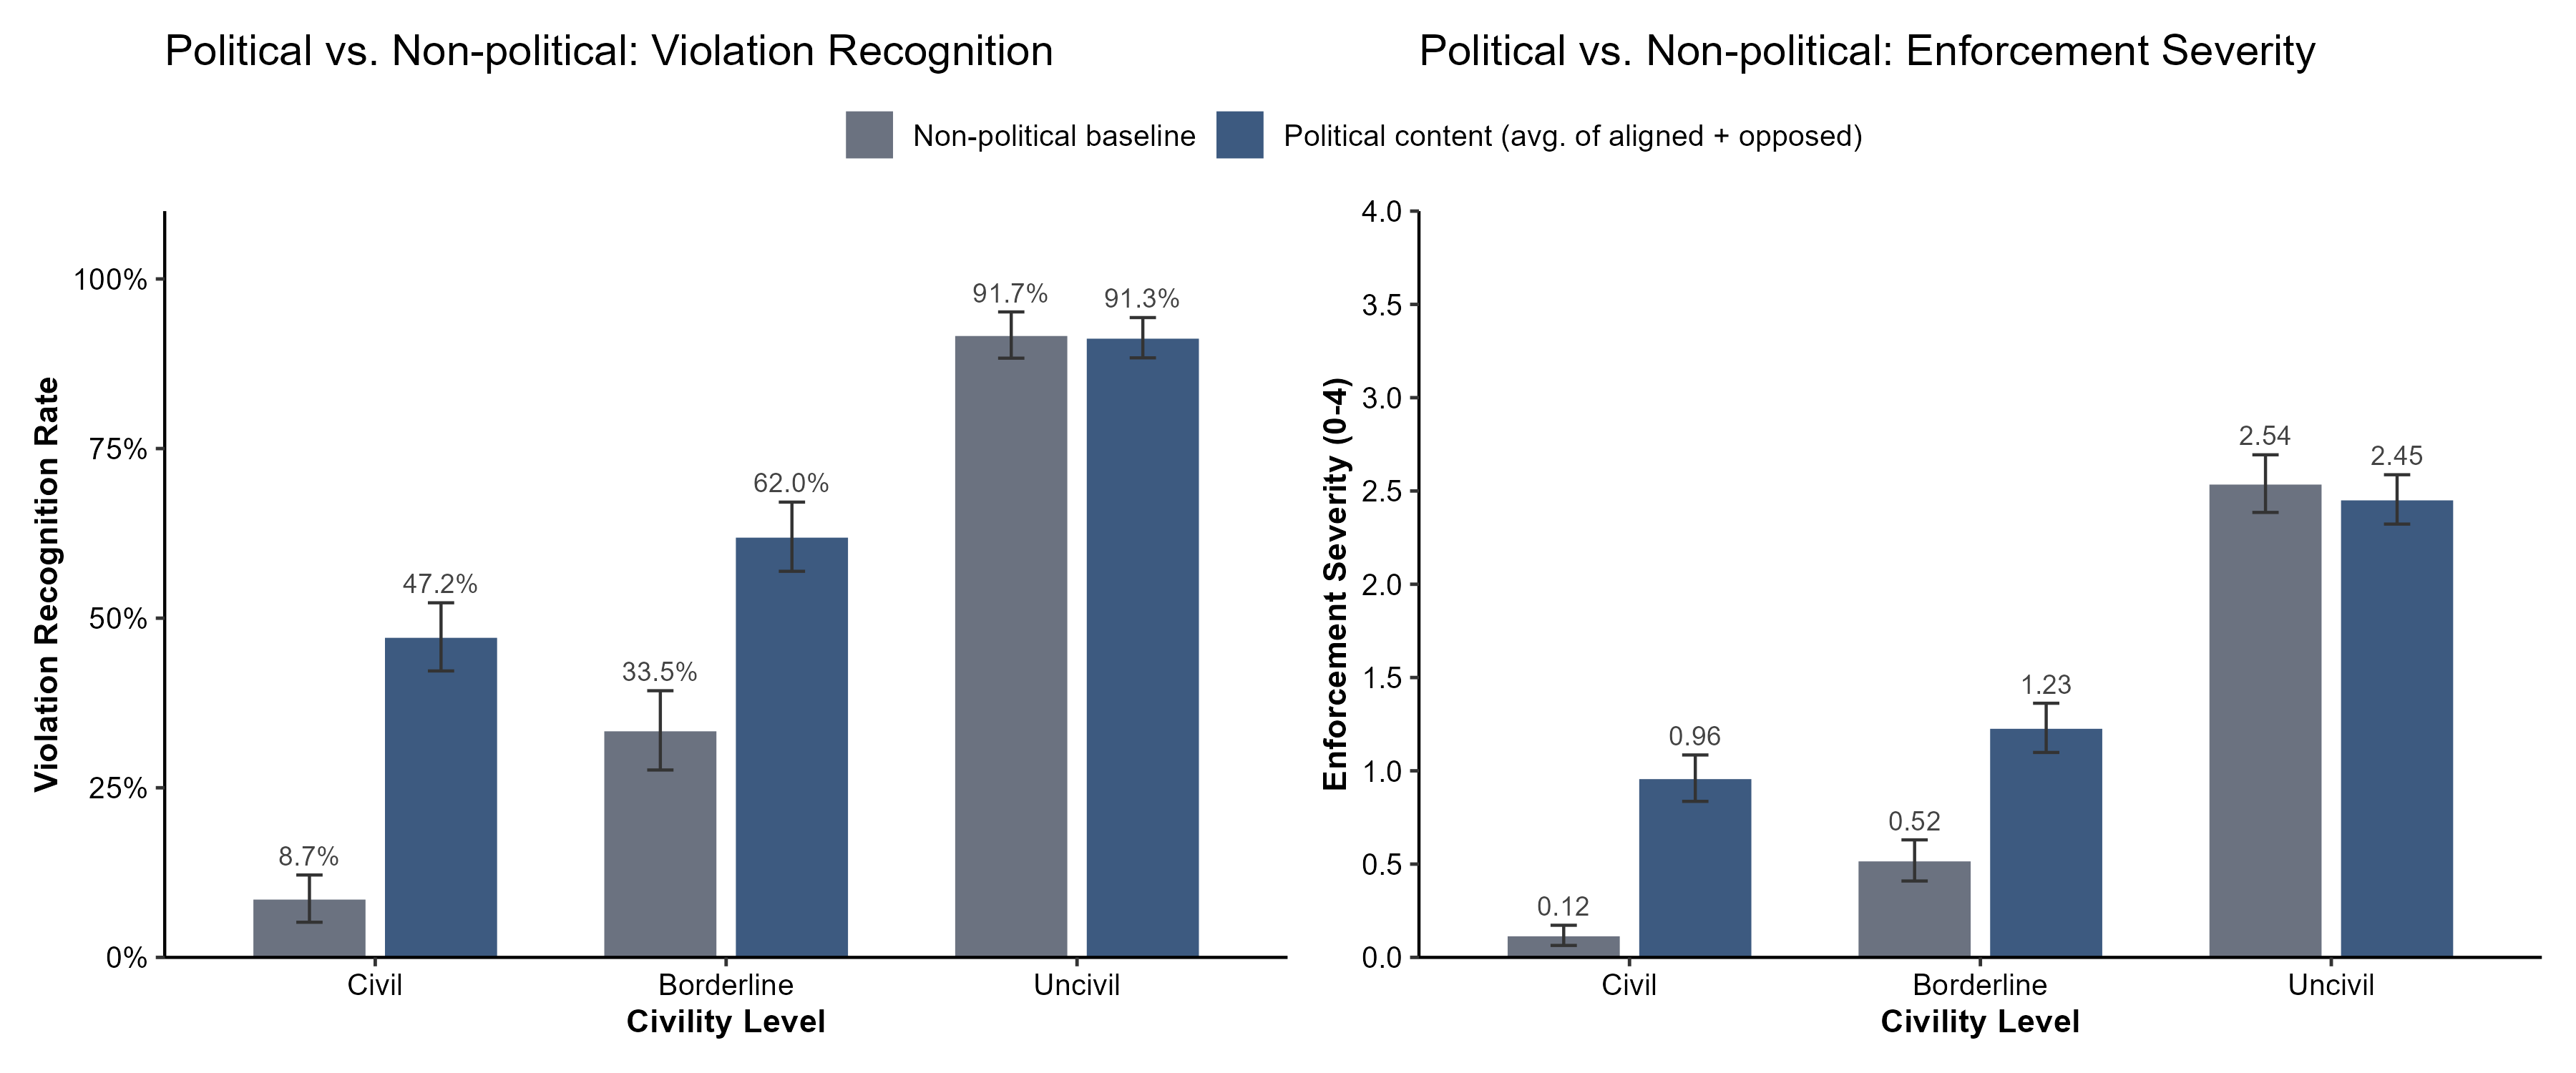
\includegraphics[width=\linewidth]{Graph_output_results/Political_vs_NonPolitical_Combined.png}
    \caption{Violation recognition and enforcement severity for political vs non-political baseline content.}
    \label{fig:nonpol_vs_pol}
\end{figure}

A similar pattern appeared for enforcement severity, which was also associated with a significant civility $\times$ content type interaction: $F(2, 506) = 73.21$, $p<0.001$, partial $\eta^2 = .224$. Political content received more severe enforcement than non-political baseline content when posts were civil ($M = 0.96$ vs.\ $0.12$, $+0.84$, $p<0.001$) or borderline uncivil ($M = 1.23$ vs.\ $0.52$, $+0.71$, $p<0.001$), but not when posts were uncivil ($M = 2.45$ vs.\ $2.54$, $p=0.19$). These findings suggest that political content is associated with more stringent moderation than non-political content at lower and borderline levels of incivility, and this distinction disappears when content is clearly uncivil.

The mechanisms underlying these patterns should be further explored, but they may highlight a general perception of political discourse as inherently contentious, even when its assigned civility level is the same. This pattern is consistent with prior work suggesting that political incivility can generate negative and heightened perceptions of conflict \parencite{mutzInYourFacePoliticsConsequences2015}. However, as the non-political posts were included as baseline items rather than as a fully randomized content-type manipulation, this comparison should be interpreted descriptively.

\subsection{Exploratory subgroup analysis: alignment effects differ across Democratic and Republican respondents}

Figure~\ref{fig:partisan_subgroup} presents civility and alignment effects on violation recognition and enforcement severity separately for Democratic ($N = 139$) and Republican ($N = 115$) respondents. This analysis is exploratory because the study was not explicitly powered to test partisan subgroup differences. Strong civility effects were observed for both groups across outcomes. For Democratic respondents, partisan alignment significantly affects violation recognition: $F(1, 138) = 12.70$, $p<0.001$, partial $\eta^2 = .084$. For Republican respondents, the alignment effect on violation recognition was not significant: $F(1, 114) = 0.98$, $p=0.324$, partial $\eta^2 = .009$. Democrats recognized violations in 60.0\% of aligned vs.\ 67.9\% of opposed cases; Republicans in 69.0\% aligned vs.\ 71.9\% opposed cases.

\begin{figure}[H]
    \centering
    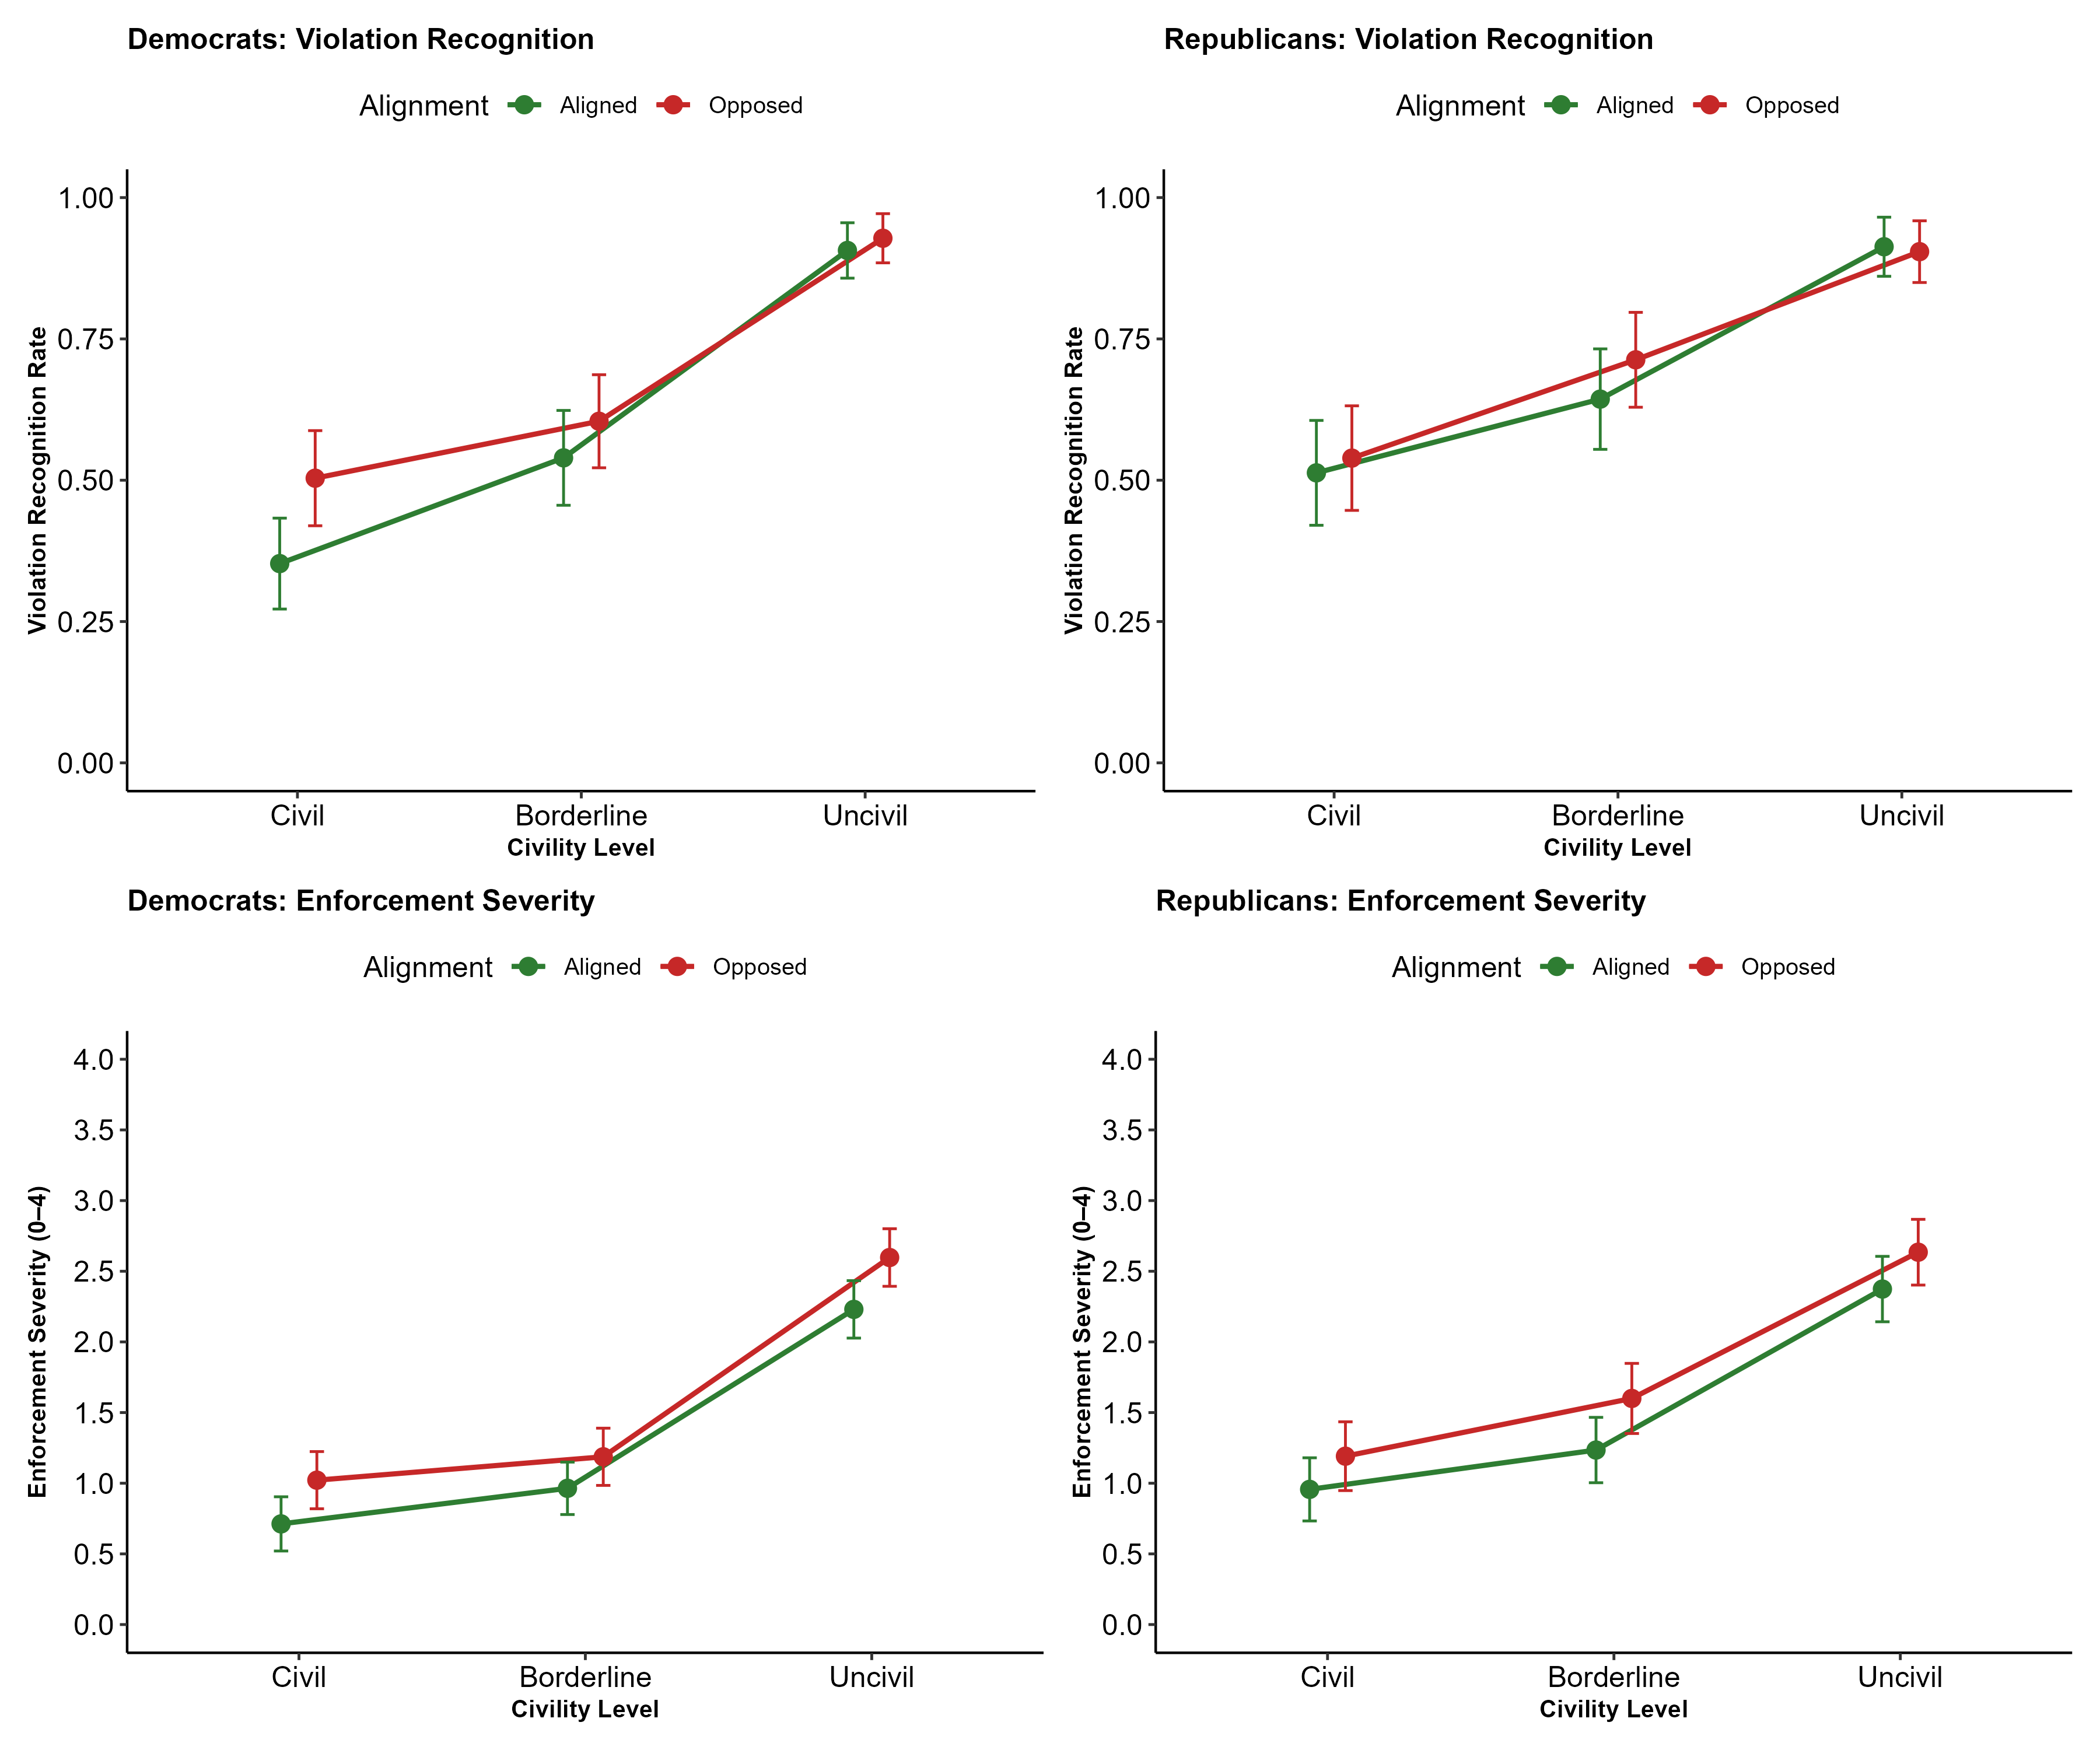
\includegraphics[width=\linewidth]{Graph_output_results/Partisan_Comparison_Plots.png}
    \caption{Violation recognition and enforcement severity by civility and alignment for political memes, Democrats vs Republicans.}
    \label{fig:partisan_subgroup}
\end{figure}

However, alignment effects were significant for both groups for enforcement severity. Democrats selected more severe actions for opposed vs.\ aligned content: $F(1, 138) = 22.53$, $p<0.001$, partial $\eta^2 = .140$; and Republicans showed the same pattern: $F(1, 114) = 11.12$, $p=0.001$, partial $\eta^2 = .089$. Democrats selected more severe actions for opposed ($M = 1.60$) than aligned content ($M = 1.30$), and the same pattern held for Republicans ($M = 1.81$ opposed vs.\ $M = 1.52$ aligned).

This suggests that alignment effects may operate differently across the two outcomes: for Democrats, alignment was associated with both recognizing violations and escalating enforcement, whereas for Republicans, it was only associated with escalating enforcement. One possible interpretation is that Republican respondents may apply a higher threshold before judging content as rule violating, perhaps signaling emphasis on free speech values \parencite{solomonIllusoryInterpartyDisagreement2024}, while still escalating enforcement once action is selected. However, results should be interpreted with caution, as small subsample sizes limit statistical power. These findings should be replicated in a design powered for between-party comparisons.

\subsection{Robustness checks: stability in studied effects across order blocks}

Figure~\ref{fig:robust_vr} presents violation recognition by civility, alignment, and order block. To assess whether the ordering approach affected the main findings, I estimated a mixed ANOVA with order block as a between-subjects factor. There was no main effect of order on violation recognition: $F(5, 248) = 0.62$, $p=0.688$, partial $\eta^2 = .012$. The main effects of civility and alignment remained significant when order was included in the model. Importantly, the order $\times$ alignment interaction was not significant: $F(5, 248) = 0.43$, $p=0.826$, partial $\eta^2 = .009$, indicating that the alignment effect on violation recognition did not meaningfully vary across blocks. The order $\times$ civility interaction was significant: $F(10, 496) = 1.90$, $p=0.043$, partial $\eta^2 = .037$, suggesting some variation in the size of the civility effect across orders. However, the overall pattern of higher violation recognition for less civil content was preserved across blocks.

\begin{figure}[H]
    \centering
    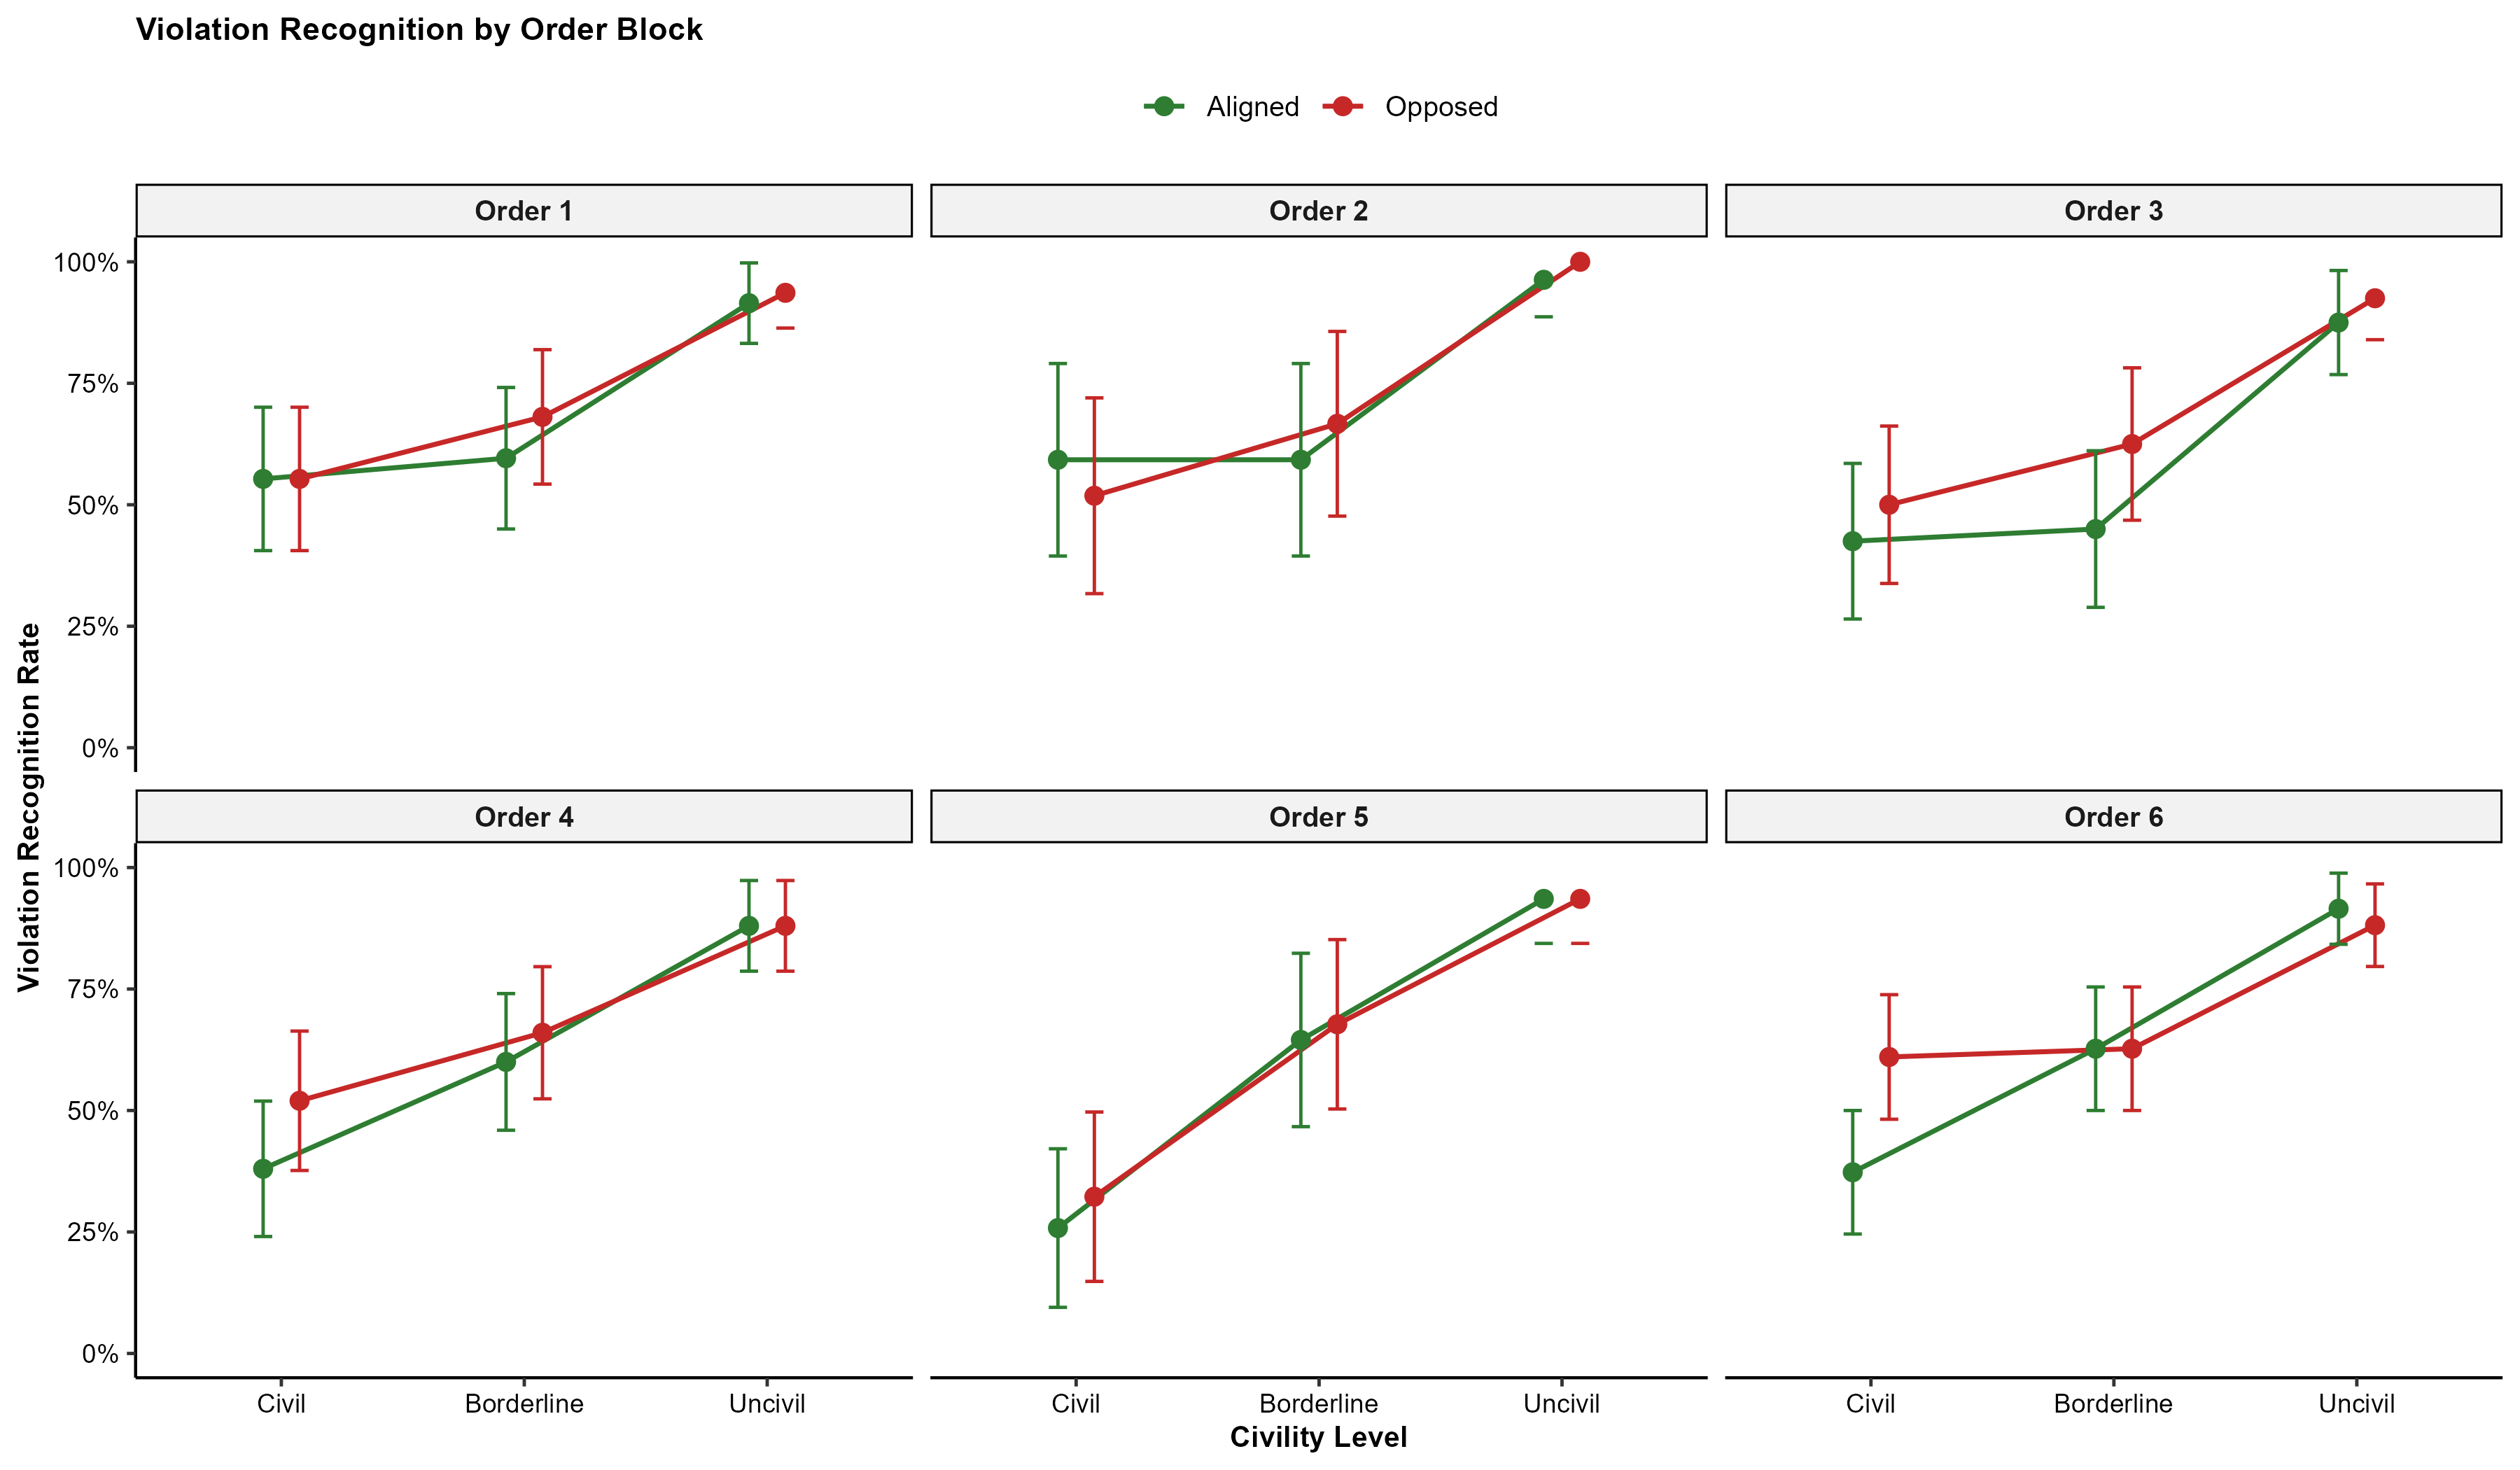
\includegraphics[width=\linewidth]{Graph_output_results/Robustness_Order_VR.png}
    \caption{Violation recognition by civility, alignment, and order block.}
    \label{fig:robust_vr}
\end{figure}

Figure~\ref{fig:robust_es} presents enforcement severity by civility, alignment and order block. There was similarly no main effect of order on enforcement severity: $F(5, 248) = 0.55$, $p=0.742$, partial $\eta^2 = .011$. The main effects of civility and alignment again remained significant, and the order $\times$ alignment interaction was again not significant: $F(5, 248) = 0.46$, $p=0.805$, partial $\eta^2 = .009$. This suggests that the alignment effect on enforcement severity was also stable across presentation orders. The three-way interaction between order, civility, and alignment was significant, suggesting some order-related variation in the joint effects of civility and alignment: $F(10, 496) = 2.50$, $p=0.006$, partial $\eta^2 = .048$. However, the central patterns---more stringent treatment of less civil content and generally stringent treatment of opposed content---remained broadly consistent across orders. Overall, the robustness checks suggest that the main conclusions of this study are not driven by presentation order, though minor order-related variations should be acknowledged.

\begin{figure}[H]
    \centering
    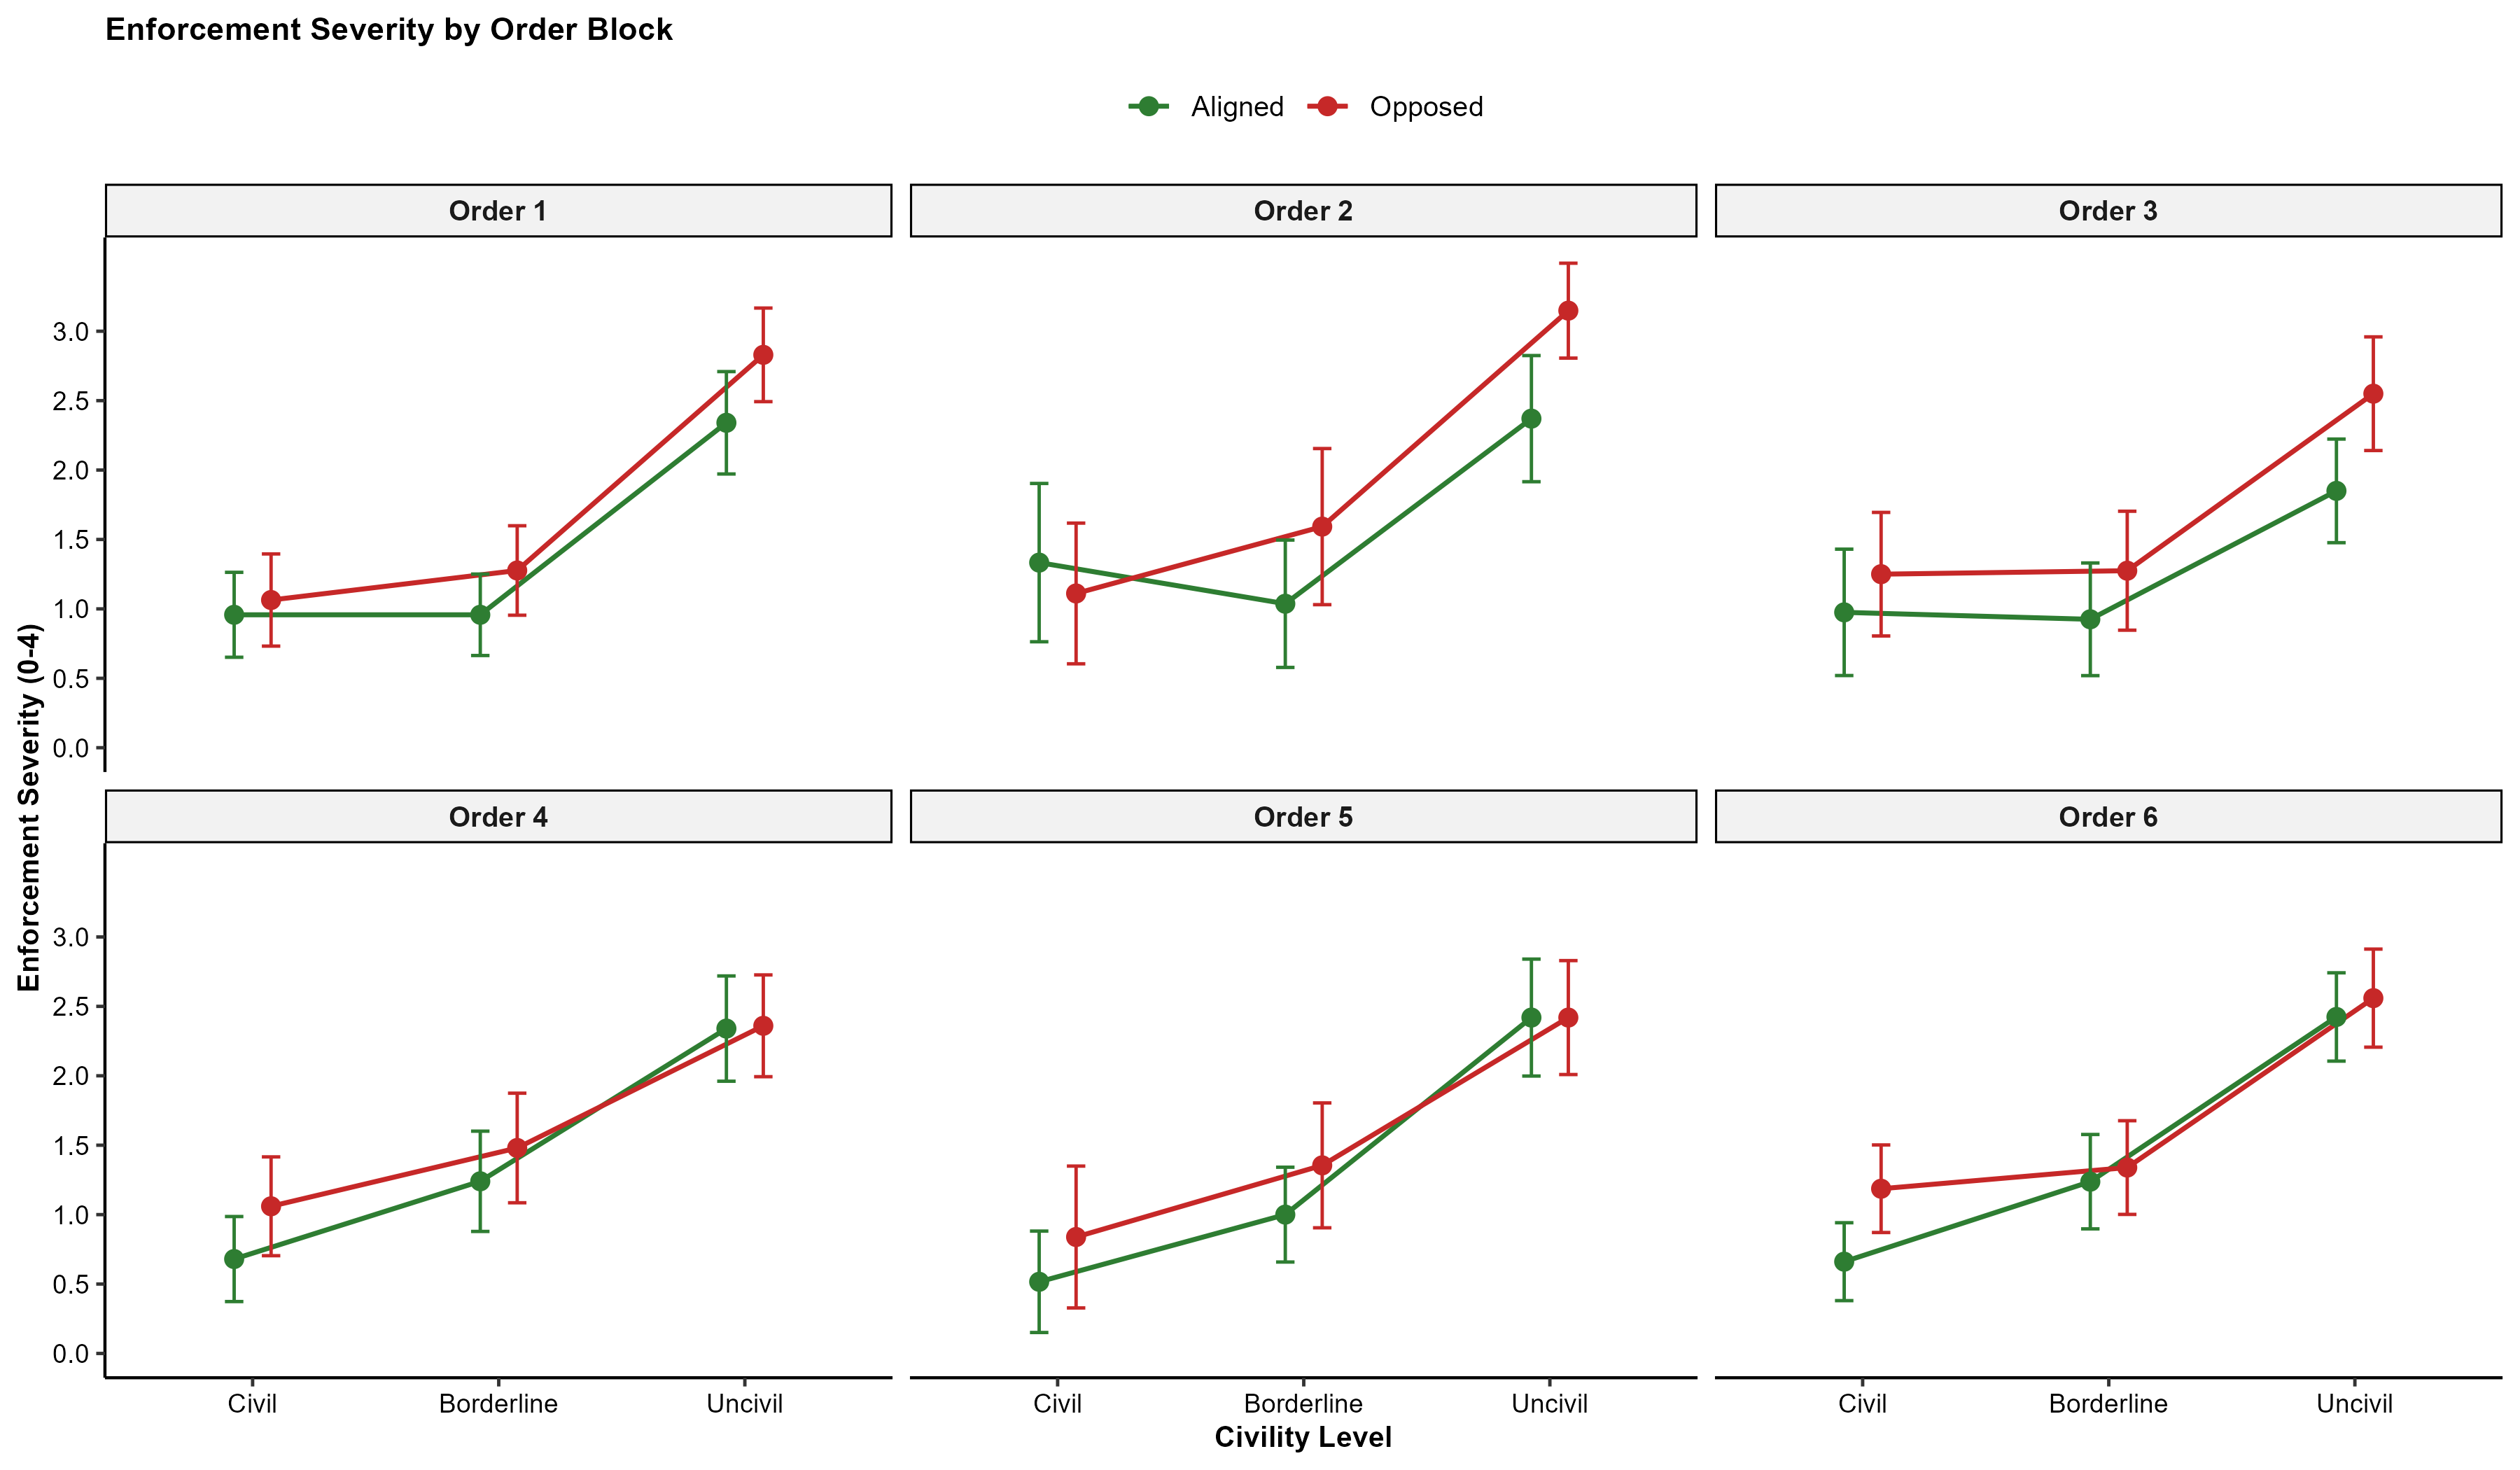
\includegraphics[width=\linewidth]{Graph_output_results/Robustness_Order_ES.png}
    \caption{Enforcement severity by civility, alignment, and order block.}
    \label{fig:robust_es}
\end{figure}

% ============================ DISCUSSION ============================
\section{Discussion}

This study provides experimental evidence of partisan alignment effects in moderation decisions. In a simulated community moderation environment, having established that respondents reliably perceive differences in incivility \textbf{(in support of H1)}, politically opposed posts were judged more often as violations of forum rules and received more severe enforcement actions \textbf{(in support of H2)}. The effect of alignment did not vary across civility levels (not supporting H3), suggesting that alignment effects were relatively uniform rather than concentrated only where content was borderline uncivil. This uniformity is substantively important, as it suggests that partisan alignment may shape moderation standards not only when rules are ambiguous, but across a broader range of civil, borderline, and uncivil political content. These findings are consistent with the \enquote{party promotion} and \enquote{preference gap} mechanisms proposed by \textcite{appelPartisanConflictContent2023a}, extending this framework from platform-level judgments about misinformation to community-level judgments about civility.

As reported above, political content was also moderated more harshly than non-political baseline content at civil and borderline levels. This pattern suggests that political content may be perceived as inherently more contentious or norm-violating than otherwise comparable non-political content. One potential mechanism is that political content generates negative affect, heightening perceptions of conflict or incivility even when the content does not clearly violate civility rules \parencite{mutzInYourFacePoliticsConsequences2015}. This finding warrants further investigation because it suggests that moderation systems may face pressures toward overcorrection of political speech, particularly where content is controversial but not clearly uncivil.

This study makes three contributions. Firstly, it extends research on politically-motivated moderation beyond fact-based evaluations, such as misinformation detection, to rule-based judgments on civility. The findings suggest that partisan alignment can shape both violation recognition and enforcement severity even when participants evaluate content against explicit community rules. Secondly, it distinguishes between two moderation outcomes: violation recognition and enforcement severity \parencite{kozyrevaResolvingContentModeration2023,solomonIllusoryInterpartyDisagreement2024}, building on prior conjoint approaches to apply these measures to a controlled within-subjects experimental design. It is important to distinguish between these outcomes because alignment effects can operate differently across judgment and enforcement, as suggested by exploratory subgroup analyses across party affiliation. Thirdly, the study examines moderation in a community forum context using meme-based stimuli, extending prior work beyond platform-level content decisions and into lower-stakes, user-governed settings where partisan content may still shape moderation behavior.

These findings inform platform governance debates. Conversations with Reddit community moderators and platform staff validated study design and suggested that online forums such as Reddit and Discord increasingly delegate moderation responsibility to volunteer communities while reducing centralized support. If similar alignment effects appear amongst volunteer moderators, communities may experience inconsistent application of rules, reducing perceptions of fairness and trust in moderation. The results point to the value of evidence-based governance interventions, including moderator training, clearer rule templates, transparent appeals processes, and platform-level audits for systematic enforcement disparities. However, the uniformity of the alignment effect across civility levels suggests that clearer rules alone may not be sufficient if participants bring stable preferences or political sensitivities to moderation decisions. Platforms should balance protection of harms from genuine incivility with preservation of legitimate political expression, especially for marginalized or under-represented communities \parencite{leesNewGenerationPerspective2022,kozyrevaResolvingContentModeration2023}.

\subsection{Limitations and further research}

Several limitations should be noted. The general U.S.\ population sample limits generalizability to actual moderators, who have more experience applying rules in real community contexts than general population respondents. Furthermore, experimental settings lack the real-world consequences of moderation which can include community backlash and reputational risks, as well as how moderators' relational knowledge of accounts in their communities may influence decision-making \parencite{taylorIdentityEffectsSocial2023}. Though prior studies suggest that content sources play a limited role in moderation decisions for U.S.\ general population respondents \parencite{kozyrevaResolvingContentModeration2023,solomonIllusoryInterpartyDisagreement2024}, conversations with moderators indicate they often use heuristics such as choice of avatar and account reputation in decision-making. This could be validated in future studies.

Furthermore, a simplified ruleset, and the limited scale and variety of content reviewed may not reflect the scale and complexity of a full moderation session. Content is restricted to ethically appropriate violations, excluding more extreme cases that moderators encounter in practice (e.g., illegal or illicit content), though such cases are likely to show less partisan divergence in practice due to clearer violation of rules or laws \parencite{kozyrevaResolvingContentModeration2023}. This study was not powered to systematically examine differences between Republican- and Democrat-aligned moderators, limiting comparisons to exploratory analysis. Prior studies focused on hate speech and misinformation suggested that Democrats may be more willing than Republicans to intervene in some moderation contexts \parencite{appelPartisanConflictContent2023a,kozyrevaResolvingContentModeration2023,solomonIllusoryInterpartyDisagreement2024}. The exploratory subgroup analysis suggests a potentially different pattern for political incivility, with Republicans displaying higher violation recognition and enforcement severity than Democrats. Additionally, the ordering approach did not fully cross all topic-condition pairings, meaning that some topics may have been paired with certain conditions more frequently across the full sample. Robustness checks suggest the main conclusions of the study are not significantly affected by presentation order. Finally, the absence of a formal pre-registration means that the analysis plan was not publicly documented prior to data collection, which limits the ability to assess potential researcher degrees of freedom, though hypotheses and analytic approach were determined before data collection began.

\subsection{Is there partisan bias?}

The study provides evidence of an alignment effect, but the term \enquote{bias} requires caution. As the study did not separately measure perceived incivility, it cannot fully distinguish whether participants applied different enforcement standards to otherwise equivalent content, or whether they perceived opposed content as genuinely more uncivil. A second interpretive challenge arises from the political vs.\ non-political comparison, because political content itself was associated with elevated moderation at civil and borderline levels, suggesting that political content may be perceived as more norm-violating or contentious even apart from alignment. The design intentionally avoided inclusion of a perceived incivility measure to reduce demand effects, but this comes at the trade-off of more limited interpretative precision.

Nevertheless, the alignment gap is meaningful. Even when content was constructed to vary systematically in incivility, opposed political content received harsher moderation judgments across the full civility range. I therefore describe the result as an alignment effect rather than definitive evidence of partisan bias. Future extensions could directly address this distinction by adding a perceived-incivility measure, whether in a moderator replication or a separate follow-up experiment.

\subsection{Extensions}

Several extensions are warranted. The most immediate is a moderator sample replication of the study, testing whether alignment effects generalize to experienced community moderators, and whether tenure, volume of posts moderated, prior training, or exposure to political forums weakens alignment effects. A follow-up experiment could also include a perceived incivility measure to distinguish whether alignment effects reflect different perceptions of the same content or different enforcement standards applied to content perceived similarly. Complementary observational analysis of real moderation decisions in political forums would test whether experiment effects generalize to naturally occurring behavior. Finally, extending the design to partisan but non-political settings, such as rivalries between sports fandoms or other identity-based groups, would help isolate whether the opposition effect reflects partisan identity per se or is specific to political content.

\subsection{Conclusion}

This study finds consistent partisan effects that increase both perceptions of content violation and consequent enforcement actions taken against uncivil content in an experiment replicating moderation in community forum settings. Alignment effects are not concentrated at borderline content, suggesting they are not driven solely by interpretative ambiguity. Moreover, political content is systematically treated more stringently than non-political content, suggesting that it may arouse a negative affect that translates to harsher judgments independent of underlying civility.

This study has important implications for both online political discourse and associated platform governance at a time when major platforms are increasingly delegating moderation to volunteer communities. If generalized population moderators exhibit alignment effects, decentralized community governance models risk proliferating enforcement disparities that undermine perceived fairness and undermine healthy democratic debate. Platforms should invest in governance, including in training, oversight, and appeals processes, in recognition that even well-intentioned moderators may struggle to apply neutral standards to political content. Future research should test whether study findings extend to moderator populations and explore evidence-based interventions to address partisan alignment.

% ============================ REFERENCES ============================
\printbibliography[title={References}]

% ============================ APPENDIX ============================
\appendix
\section{Appendix}

\subsection{Descriptive Statistics}
\label{sec:descriptive}

Table~\ref{tab:descriptive} below presents descriptive statistics for demographic characteristics and political party alignment across the six counterbalancing blocks. Political affiliation was well-distributed with Democrats comprising 48.1--61\% and Republicans comprising 39.0--51.9\% of the sample across blocks. Age, ethnicity, education level and employment status are also summarized by block to describe the sample composition. These descriptive statistics are provided for transparency and are not a formal test of randomization balance.

% -------- TABLE 2: Descriptive statistics --------
{%
\footnotesize
\setlength{\tabcolsep}{4pt}
\renewcommand{\arraystretch}{1.12}

\begin{xltabular}{\textwidth}{@{}
  >{\raggedright\arraybackslash}p{2.2cm}
  >{\raggedright\arraybackslash}X
  >{\centering\arraybackslash}p{1.0cm}
  >{\centering\arraybackslash}p{0.75cm}
  >{\centering\arraybackslash}p{0.75cm}
  >{\centering\arraybackslash}p{0.75cm}
  >{\centering\arraybackslash}p{0.75cm}
  >{\centering\arraybackslash}p{0.75cm}
  >{\centering\arraybackslash}p{0.75cm}
@{}}

\caption{Descriptive statistics on political party preference and demographics.}
\label{tab:descriptive}\\[-2pt]

\toprule
\textbf{Field} & \textbf{Category} & \textbf{Whole} & \textbf{O1} & \textbf{O2} & \textbf{O3} & \textbf{O4} & \textbf{O5} & \textbf{O6} \\
\midrule
\endfirsthead

\multicolumn{9}{@{}l@{}}{\textit{Table~\ref{tab:descriptive} continued from previous page}}\\[2pt]
\toprule
\textbf{Field} & \textbf{Category} & \textbf{Whole} & \textbf{O1} & \textbf{O2} & \textbf{O3} & \textbf{O4} & \textbf{O5} & \textbf{O6} \\
\midrule
\endhead

\midrule
\multicolumn{9}{r}{\textit{Continued on next page\ldots}}\\
\endfoot

\bottomrule
\endlastfoot

Block size & --- & 254 & 47 & 27 & 40 & 31 & 50 & 59 \\
\midrule

Political leaning & Democrat (n) & 139 & 23 & 13 & 22 & 17 & 28 & 36 \\
                  & Democrat (\%) & 54.7 & 48.9 & 48.1 & 55.0 & 54.8 & 56.0 & 61.0 \\
                  & Republican (n) & 115 & 24 & 14 & 18 & 14 & 22 & 23 \\
                  & Republican (\%) & 45.3 & 51.1 & 51.9 & 45.0 & 45.2 & 44.0 & 39.0 \\
\midrule

Age & Mean & 47.0 & 44.8 & 46.0 & 51.8 & 46.8 & 44.3 & 48.6 \\
\midrule

Ethnicity & White/Caucasian (n) & 187 & 33 & 19 & 31 & 24 & 38 & 42 \\
          & Black/African American (n) & 35 & 4 & 3 & 6 & 3 & 5 & 14 \\
          & Asian (n) & 12 & 2 & 2 & 2 & 2 & 4 & 0 \\
          & American Indian/Alaska Native (n) & 2 & 1 & 0 & 0 & 0 & 0 & 1 \\
          & Other race/ethnicity (n) & 16 & 6 & 3 & 1 & 1 & 3 & 2 \\
          & Prefer not to answer (n) & 2 & 1 & 0 & 0 & 1 & 0 & 0 \\
\midrule

Education & Less than high school graduate (n) & 4 & 0 & 0 & 3 & 0 & 1 & 0 \\
          & High school graduate/GED (n) & 46 & 13 & 4 & 6 & 4 & 10 & 9 \\
          & Some college, no degree (n) & 45 & 7 & 7 & 4 & 3 & 10 & 14 \\
          & Trade/technical training (n) & 9 & 0 & 3 & 0 & 0 & 2 & 4 \\
          & Associate degree (n) & 34 & 7 & 2 & 10 & 5 & 4 & 6 \\
          & Bachelor's degree (n) & 78 & 12 & 8 & 11 & 14 & 17 & 16 \\
          & Master's degree (n) & 34 & 6 & 3 & 6 & 3 & 6 & 10 \\
          & Professional degree (n) & 2 & 1 & 0 & 0 & 1 & 0 & 0 \\
          & Doctorate degree (n) & 2 & 1 & 0 & 0 & 1 & 0 & 0 \\
\midrule

Employment & Full time (n) & 120 & 29 & 11 & 16 & 16 & 22 & 26 \\
           & Part time (n) & 32 & 2 & 6 & 5 & 4 & 6 & 9 \\
           & Retired (n) & 40 & 5 & 3 & 9 & 6 & 8 & 9 \\
           & Homemaker (n) & 12 & 1 & 1 & 3 & 3 & 3 & 1 \\
           & Student (n) & 17 & 2 & 2 & 1 & 0 & 4 & 8 \\
           & Other (n) & 11 & 3 & 2 & 2 & 0 & 2 & 2 \\
           & Unemployed, seeking work (n) & 12 & 3 & 0 & 2 & 1 & 4 & 2 \\
           & Unemployed, not seeking work (n) & 10 & 2 & 2 & 2 & 1 & 1 & 2 \\

\end{xltabular}
}%

\noindent\textit{Note:} O1--O6 denote order blocks 1 through 6. Percentages for ethnicity, education, and employment categories are omitted for compactness; counts are shown.

\subsection{Study material exhibits}

\begin{figure}[H]
    \centering
    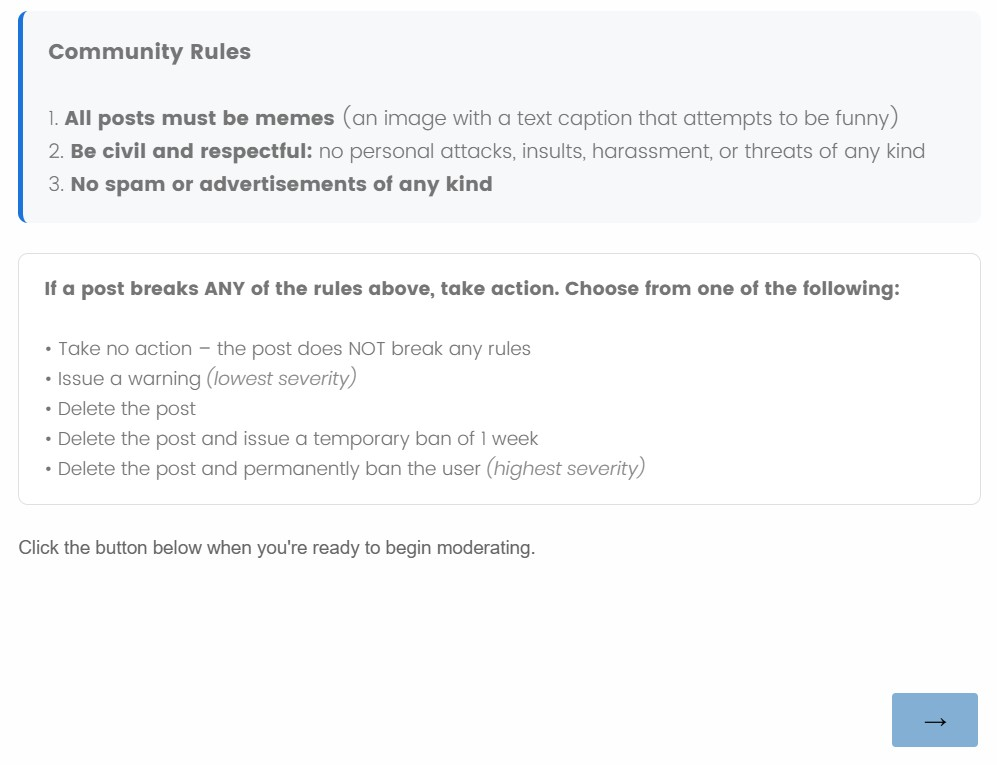
\includegraphics[width=\linewidth]{Study_Exhibits/Fig_8_Community_Rules.jpg}
    \caption{Community forum rules and moderation instructions (displayed to participants).}
    \label{fig:comm_rules}
\end{figure}

\begin{figure}[H]
    \centering
    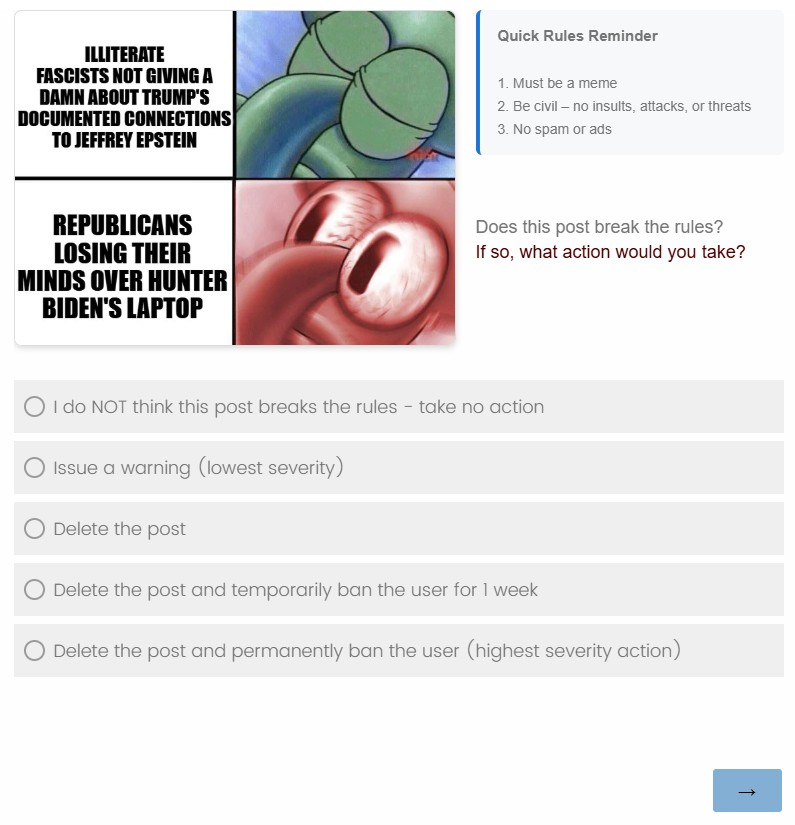
\includegraphics[width=\linewidth]{Study_Exhibits/Fig_9_Example_Question_Screen.jpg}
    \caption{Community forum rules and moderation instructions (displayed to participants).}
    \label{fig:question_screen}
\end{figure}

\begin{figure}[H]
    \centering
    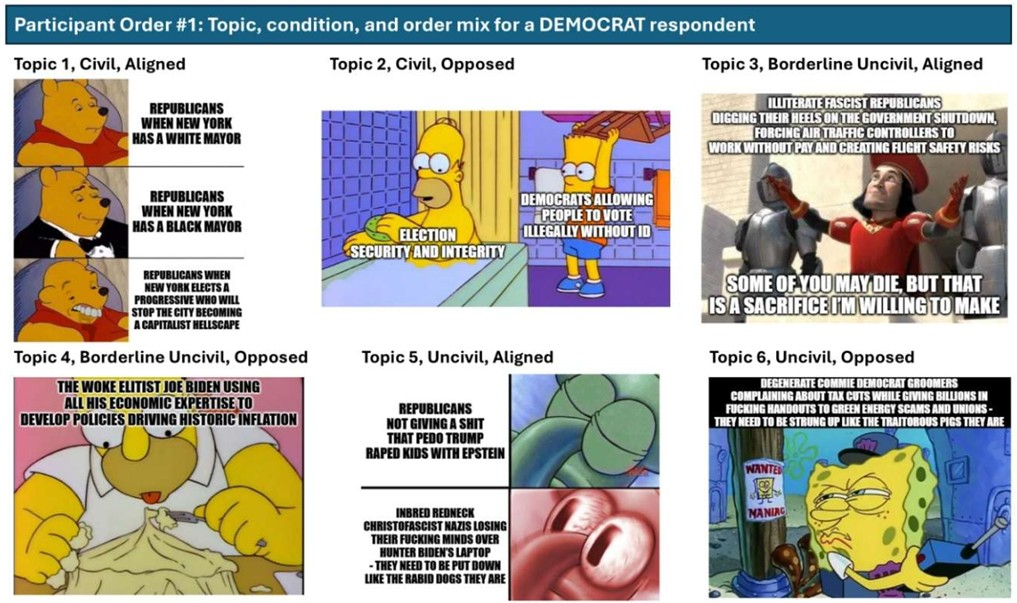
\includegraphics[width=\linewidth]{Study_Exhibits/Fig_10_Example_Topic_Order_Condition.jpg}
    \caption{Example topic, order, and condition mix for a respondent (Participant Order \#1).\protect\footnotemark}
    \label{fig:ordermix}
\end{figure}
\footnotetext{As the participant is a Democrat (i.e., left-aligned), \enquote{left-aligned} posts map to \enquote{aligned} conditions, and \enquote{right-aligned} posts map to \enquote{opposed} conditions. Partisan alignment for the same set of memes would be reversed for Republican respondents.}

\begin{figure}[H]
    \centering
    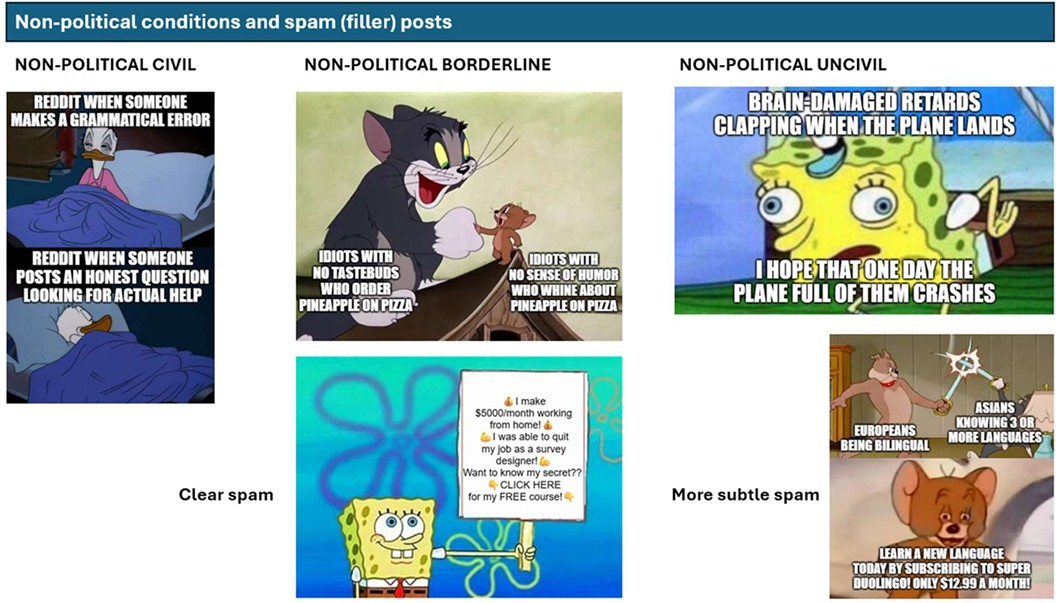
\includegraphics[width=\linewidth]{Study_Exhibits/Fig_11_Non_Political_Spam.jpg}
    \caption{Non-political baseline and filler memes, presented to all participants.}
    \label{fig:spam_nonpol}
\end{figure}

% -------- TABLE 3: Full meme list --------
{%
\small
\setlength{\tabcolsep}{5pt}
\setlength{\LTleft}{0pt}
\setlength{\LTright}{0pt}
\setlength{\LTcapwidth}{\textwidth}

\begin{longtable}{@{} 
  >{\centering\arraybackslash}p{0.9cm}
  >{\raggedright\arraybackslash}p{3.0cm}
  >{\centering\arraybackslash}p{1.7cm}
  >{\raggedright\arraybackslash}p{\dimexpr\textwidth-0.9cm-3.0cm-1.7cm-6\tabcolsep\relax}
@{}}

\caption{Full list of memes, topics, and conditions by order block.}
\label{tab:memes}\\[-2pt]

\multicolumn{4}{@{}l@{}}{\textit{L = left-leaning; R = right-leaning; Bord.\ = borderline uncivil}}\\[4pt]

\toprule
\textbf{Order} & \textbf{Topic / meme} & \textbf{Cond.} & \textbf{Meme content} \\
\midrule
\endfirsthead

% ----- ORDER 1 -----
1 & Mamdani; Pooh       & Civil-L    & ``Republicans when NY Has a White Mayor'' / ``Republicans when NY has a Black Mayor'' / ``Republicans when NY elects a progressive who will stop the city becoming a capitalist hellscape'' \\[2pt]
1 & Election sec.; Simpsons & Civil-R & Homer: ``Election security and integrity''; Bart: ``Democrats allowing people to vote illegally without ID'' \\[2pt]
1 & Gov.\ shutdown; Farquaad & Bord.-L & ``Illiterate fascist Republicans digging their heels on the government shutdown, forcing air traffic controllers to work without pay and creating flight safety risks'' / ``Some of you may die, but that is a sacrifice I'm willing to make'' \\[2pt]
1 & Economy; Simpsons   & Bord.-R   & ``The woke elitist Joe Biden using all his economic expertise to develop policies driving historic inflation'' \\[2pt]
1 & Laptop/Epstein; Spongebob & Uncivil-L & ``Republicans not giving a shit that pedo Trump raped kids with Epstein'' / ``Inbred redneck Christofascist Nazis losing their fucking minds over Hunter Biden's laptop --- they need to be put down like the rabid dogs they are'' \\[2pt]
1 & Green energy; Spongebob & Uncivil-R & ``Degenerate commie Democrat groomers complaining about tax cuts while giving billions in fucking handouts to green energy scams and unions --- they need to be strung up like the traitorous pigs they are'' \\
\midrule

% ----- ORDER 2 -----
2 & Gov.\ shutdown; Farquaad & Civil-R & ``Democrats digging their heels in with the government shutdown, forcing air traffic controllers to work without pay and creating flight safety risks'' / ``Some of you may die, but that is a sacrifice I'm willing to make'' \\[2pt]
2 & Economy; Simpsons   & Bord.-L   & ``The illiterate fascist Donald Trump using all his business experience to come up with devastatingly stupid tariffs'' \\[2pt]
2 & Laptop/Epstein; Spongebob & Bord.-R & ``Woke elitists not giving a damn when Hunter Biden's laptop shows clear evidence of corruption'' / ``Democrats losing their minds when they hear Trump was photographed with Epstein'' \\[2pt]
2 & Green energy; Spongebob & Uncivil-L & ``Inbred redneck Christofascist Nazi Republicans looking to cut government spending while giving billions in fucking handouts to corporate donors --- they need to be put down like the rabid dogs they are'' \\[2pt]
2 & Mamdani; Pooh       & Uncivil-R  & ``New York Has a White Mayor'' / ``New York has a Black Mayor'' / ``New York just elected a terrorist and degenerate commie groomers are celebrating --- they need to be strung up like the traitorous pigs they are'' \\[2pt]
2 & Election sec.; Simpsons & Civil-L & Homer: ``Marginalized communities' right to vote''; Bart: ``Voter ID laws introduced by Republicans'' \\
\midrule

% ----- ORDER 3 -----
3 & Laptop/Epstein; Spongebob & Bord.-L & ``Illiterate fascists not giving a damn about Trump's documented connections to Jeffrey Epstein'' / ``Republicans losing their minds over Hunter Biden's laptop'' \\[2pt]
3 & Green energy; Spongebob & Bord.-R & ``Woke elitist Democrats complaining about tax cuts while giving billions in subsidies to green energy companies and unions'' \\[2pt]
3 & Mamdani; Pooh       & Uncivil-L  & ``Republicans when NY Has a White Mayor'' / ``Republicans when NY has a Black Mayor'' / ``Inbred redneck Christofascist Nazis having a total meltdown because NY elected a progressive --- they need to be put down like the rabid dogs they are'' \\[2pt]
3 & Election sec.; Simpsons & Uncivil-R & Homer: ``Election security and integrity''; Bart: ``Democrats letting illegals commit voter fraud --- these degenerate commie groomers need to be strung up like the traitorous pigs they are'' \\[2pt]
3 & Gov.\ shutdown; Farquaad & Civil-L & ``Republicans digging their heels in with the government shutdown, forcing air traffic controllers to work without pay and creating flight safety risks'' / ``Some of you may die, but that is a sacrifice I'm willing to make'' \\[2pt]
3 & Economy; Simpsons   & Civil-R   & ``Joe Biden using all his economic expertise to develop policies driving historic inflation'' \\
\midrule

% ----- ORDER 4 -----
4 & Mamdani; Pooh       & Bord.-R    & ``New York Has a White Mayor'' / ``New York has a Black Mayor'' / ``New York just elected a communist and woke elitist Democrats are celebrating'' \\[2pt]
4 & Election sec.; Simpsons & Uncivil-L & Homer: ``Marginalized communities' right to vote''; Bart: ``Voter ID laws introduced by Republicans --- these inbred redneck Christofascist Nazis need to be put down like the rabid dogs they are'' \\[2pt]
4 & Gov.\ shutdown; Farquaad & Uncivil-R & ``Degenerate commie Democrat groomers digging in their heels on the shutdown, risking plane crashes to protect their illegal voters --- any planes that go down should take these traitorous pigs with them'' / ``Some of you may die, but that is a sacrifice I'm willing to make'' \\[2pt]
4 & Economy; Simpsons   & Civil-L   & ``Donald Trump using all his business experience to develop economically harmful tariff policies'' \\[2pt]
4 & Laptop/Epstein; Spongebob & Civil-R & ``Democrats when Hunter Biden's laptop shows clear evidence of corruption'' / ``Democrats when they hear Trump was photographed with Epstein'' \\[2pt]
4 & Green energy; Spongebob & Bord.-L & ``Illiterate fascist Republicans looking to cut government spending while giving billions in corporate welfare to their donors'' \\
\midrule

% ----- ORDER 5 -----
5 & Gov.\ shutdown; Farquaad & Uncivil-L & ``Inbred redneck Christofascist Nazi Republicans digging in their heels on the shutdown, risking plane crashes just to own the libs --- any planes that go down should take these rabid dogs with them'' / ``Some of you may die, but that is a sacrifice I'm willing to make'' \\[2pt]
5 & Economy; Simpsons   & Uncivil-R  & ``The senile piece of shit Joe Biden pushing devastatingly stupid policies driving inflation --- he and his band of degenerate commie groomers need to be strung up like the traitorous pigs they are'' \\[2pt]
5 & Laptop/Epstein; Spongebob & Civil-L & ``Republicans when they hear Trump has documented connections to Jeffrey Epstein'' / ``Republicans when they hear rumors about Hunter Biden's laptop'' \\[2pt]
5 & Green energy; Spongebob & Civil-R  & ``Woke elitist Democrats complaining about tax cuts while giving billions in subsidies to green energy companies and unions'' \\[2pt]
5 & Mamdani; Pooh       & Bord.-L    & ``Republicans when NY Has a White Mayor'' / ``Republicans when NY has a Black Mayor'' / ``Illiterate fascists losing their minds when New York elects a progressive'' \\[2pt]
5 & Election sec.; Simpsons & Bord.-R & Homer: ``Election security and integrity''; Bart: ``Voter ID laws opposed by woke elitist Democrats letting illegals vote'' \\
\midrule

% ----- ORDER 6 -----
6 & Laptop/Epstein; Spongebob & Uncivil-R & ``Democrats not giving a shit about Hunter Biden and the Biden crime family selling America to China'' / ``Degenerate commie groomers losing their fucking minds over Trump being photographed with Epstein --- they need to be strung up like the traitorous pigs they are'' \\[2pt]
6 & Green energy; Spongebob & Civil-L  & ``Republicans looking to cut government spending while giving billions in corporate welfare to their donors'' \\[2pt]
6 & Mamdani; Pooh       & Civil-R    & ``New York Has a White Mayor'' / ``New York has a Black Mayor'' / ``New York just elected a radical leftist who will create a socialist hellscape'' \\[2pt]
6 & Election sec.; Simpsons & Bord.-L & ``Marginalized communities' right to vote'' / ``Voter ID laws introduced by illiterate fascist Republicans'' \\[2pt]
6 & Gov.\ shutdown; Farquaad & Bord.-R & ``Woke elitist Democrats digging their heels in with the government shutdown, forcing air traffic controllers to work without pay and creating flight safety risks'' / ``Some of you may die, but that is a sacrifice I'm willing to make'' \\[2pt]
6 & Economy; Simpsons   & Uncivil-L  & ``The senile piece of shit Donald Trump pushing devastatingly stupid tariffs --- he and his band of inbred Christofascist rednecks need to be put down like the rabid dogs they are'' \\

\end{longtable}
}%

\end{document}
